\documentclass[pl,12pt]{aghdpl}
% \documentclass[en,11pt]{aghdpl}  % praca w języku angielskim

% Lista wszystkich języków stanowiących języki pozycji bibliograficznych użytych w pracy.
% (Zgodnie z zasadami tworzenia bibliografii każda pozycja powinna zostać utworzona zgodnie z zasadami języka, w którym dana publikacja została napisana.)
\usepackage[english,polish]{babel}

% Użyj polskiego łamania wyrazów (zamiast domyślnego angielskiego).
\usepackage{polski}

\usepackage[utf8]{inputenc}

% Załączniki

\usepackage[toc, page]{appendix}
\renewcommand\appendixpagename{Załączniki}
\renewcommand\appendixtocname{Załączniki}

% dodatkowe pakiety

\usepackage{mathtools}
\usepackage{amsfonts}
\usepackage{amsmath}
\usepackage{amsthm}
\usepackage{float}% do umieszczenia floatów [H]
\usepackage{enumitem}
\setlist{nosep} % or \setlist{noitemsep} to leave space around whole list
\usepackage[bookmarks,hidelinks]{hyperref}

% Środowisko float do kodu źródłowego \begin{program}

\floatstyle{plaintop}
\ifcsname{chapter}\endcsname%
    \newfloat{program}{!tbh}{lop}[chapter]
\else%
    \newfloat{program}{!tbh}{lop}
\fi
\floatname{program}{Kod źr.}

% Kod poniżej powoduje, że floaty nie wylatują poza granice sekcji

\usepackage{placeins}

\ifcsname{chapter}\endcsname%
    \let\Oldchapter\chapter%
    \renewcommand{\chapter}{\FloatBarrier\Oldchapter}
\fi

\let\Oldsection\section%
\renewcommand{\section}{\FloatBarrier\Oldsection}

\let\Oldsubsection\subsection%
\renewcommand{\subsection}{\FloatBarrier\Oldsubsection}

\let\Oldsubsubsection\subsubsection%
\renewcommand{\subsubsection}{\FloatBarrier\Oldsubsubsection}

% --- < bibliografia > ---


\usepackage[
style=numeric,
sorting=none,
%
% Zastosuj styl wpisu bibliograficznego właściwy językowi publikacji.
language=autobib,
autolang=other,
% Zapisuj datę dostępu do strony WWW w formacie RRRR-MM-DD.
urldate=iso,
seconds=true,
% Nie dodawaj numerów stron, na których występuje cytowanie.
backref=false,
% Podawaj ISBN.
isbn=true,
% Nie podawaj URL-i, o ile nie jest to konieczne.
url=false,
%
% Ustawienia związane z polskimi normami dla bibliografii.
maxbibnames=3,
% Jeżeli używamy Bibera:
backend=bibtex
]{biblatex}

\usepackage{csquotes}
% Ponieważ `csquotes` nie posiada polskiego stylu, można skorzystać z mocno zbliżonego stylu chorwackiego.
\DeclareQuoteAlias{croatian}{polish}

\addbibresource{bibliografia.bib}

% Przecinki zamiast kropek do oddzielenia pól wpisu bibliograficznego
% i dwukropek po nazwisku autora, bez kropki na końcu
\AtBeginBibliography{
    \renewcommand\labelnamepunct{:\space}
    \renewcommand\newunitpunct{\addcomma\space}
    \renewcommand{\finentrypunct}{}
    
    \renewcommand{\bibopenparen}{\addcomma\addspace}
    \renewcommand{\bibcloseparen}{\addspace}
}

% Nie wyświetlaj wybranych pól.
%\AtEveryBibitem{\clearfield{note}}


% ------------------------
% --- < listingi > ---

% Użyj czcionki kroju Times.
\usepackage{newtxtext}
\usepackage{newtxmath}

\usepackage{listings}
\lstset{language=TeX}

\lstset{%
        literate={ą}{{\k{a}}}1
           {ć}{{\'c}}1
           {ę}{{\k{e}}}1
           {ó}{{\'o}}1
           {ń}{{\'n}}1
           {ł}{{\l{}}}1
           {ś}{{\'s}}1
           {ź}{{\'z}}1
           {ż}{{\.z}}1
           {Ą}{{\k{A}}}1
           {Ć}{{\'C}}1
           {Ę}{{\k{E}}}1
           {Ó}{{\'O}}1
           {Ń}{{\'N}}1
           {Ł}{{\L{}}}1
           {Ś}{{\'S}}1
           {Ź}{{\'Z}}1
           {Ż}{{\.Z}}1
}

% Ustawienia pakietu lstlisting do umieszczania kodu

\usepackage{color}

\definecolor{mygreen}{rgb}{0,0.6,0}
\definecolor{mygray}{rgb}{0.5,0.5,0.5}
\definecolor{mymauve}{rgb}{0.58,0,0.82}

\lstset{%
  backgroundcolor=\color{white},     % choose the background color
  basicstyle=\ttfamily\footnotesize, % size of fonts used for the code
  breaklines, breakatwhitespace,     % automatic line breaking only at whitespace
  commentstyle=\color{mygreen},      % comment style
  numbers=left,
  showstringspaces=false,
  numberstyle=\tiny,
  frame=l,
  escapeinside={*@}{@*},           % if you want to add LaTeX within your code
  keywordstyle=\color{blue},         % keyword style
  stringstyle=\color{mymauve}        % string literal style
}

% ------------------------

\AtBeginDocument{%
        \renewcommand{\tablename}{Tab.}
        \renewcommand{\figurename}{Rys.}
}

% ------------------------
% --- < tabele > ---

\usepackage{array}
\usepackage{tabularx}
\usepackage{multirow}
\usepackage{booktabs}
\usepackage{makecell}
\usepackage[flushleft]{threeparttable}

% defines the X column to use m (\parbox[c]) instead of p (`parbox[t]`)
\newcolumntype{C}[1]{>{\hsize=#1\hsize\centering\arraybackslash}X}


%---------------------------------------------------------------------------

\author{{Dominik Szymaniak}}

\makeatletter% Poniższe makra są wyłącznie zdefiniowane w klasie aghdpl-imir
\@ifclassloaded{aghdpl}{%

  \sex{m} % Rodzaj osobowych form czasowników: m - męski, ż - żeński
  \shortauthor{{D.\ Szymaniak}}
  \albumnum{{269564}}
  \address{{[Adres]}}

  \titlePL{{Zastosowanie procesorów graficznych do obliczeń akustycznych}}
  \titleEN{{Implementation of graphics processing units for acoustic calculations}}

  \shorttitlePL{{Zastosowanie procesorów graficznych do obliczeń akustycznych}} % skrócona wersja tytułu
  \shorttitleEN{{Implementation of graphics processing units for acoustic calculations}}

  % rodzaj pracy bez końcówki fleksyjnej np. inżyniersk, magistersk
  \thesistypePL{magistersk}
  \thesistypeEN{engineer}

  \supervisor{{dr Marek Pluta}}

  \reviewer{{dr hab. Inż. Mariusz Giergiel, prof. AGH}}

  \degreeprogrammePL{{Inżynieria Akustyczna}}
  \degreeprogrammeEN{{Acoustic Engineering}}

  \specialisationPL{{Drgania i Hałas w Technice i Środowisku (D)}}
  \specialisationEN{{[Specialisation]}}

  \graduationyear{{2019}}
  \years{2018/2019}
  \yearofstudy{IV}
  \formPL{stacjonarne}
  \formEN{full-time}

  % zgoda na publikację pracy w internecie: t-zgoda, cokolwiek 
  % innego-brak zgody
  \agree{t}

  % praktyka (dyplomowa)
  \apprenticeship{{[Praktyka dyplomowa]}}

  \department{Katedra Transportu Linowego}

  \facultyPL{Wydział Inżynierii Mechanicznej i Robotyki}
  \facultyEN{Faculty of Mechanical Engineering and Robotics}

  \thesisplan{% Przykładowy plan pracy, należy omówić z promotorem
    \begin{enumerate}
    \item Omówienie tematu pracy i sposobu realizacji z promotorem.
    \item Zebranie i opracowanie literatury dotyczącej tematu pracy.
    \item Zebranie i opracowanie wyników badań.
    \item Analiza wyników badań, ich omówienie i zatwierdzenie przez promotora.
    \item Opracowanie redakcyjne.
    \end{enumerate}
  }

  \summaryPL{\indent\indent%
	  {[Treść streszczenia]}
  }
  \summaryEN{\indent\indent%
	  {[Summary text]}
  }

  \acknowledgements{%
    "Więc z punktu, mając na uwadze,\\*
 że ewentualna krytyka może być...\\*
 tak musimy zrobić, \\* żeby tej krytyki nie było...\\*
 tylko aplauz i zaakceptowanie (...)"\\*
- "Rejs" M. Piwowskiego
  }

  \setlength{\cftsecnumwidth}{10mm}
}{}%
\makeatother%

\date{\today}

%---------------------------------------------------------------------------
\setcounter{secnumdepth}{4}
\brokenpenalty=10000\relax


\begin{document}

\titlepages{}

% Ponowne zdefiniowanie stylu `plain`, aby usunąć numer strony z pierwszej strony spisu treści i poszczególnych rozdziałów.
\fancypagestyle{plain}
{%
        % Usuń nagłówek i stopkę
        \fancyhf{}
        % Usuń linie.
        \renewcommand{\headrulewidth}{0pt}
        \renewcommand{\footrulewidth}{0pt}
}

\setcounter{tocdepth}{2}
{\singlespacing\tableofcontents}
\clearpage

\chapter{Wprowadzenie}\label{cha:wprowadzenie}

\LaTeX~jest systemem składu umożliwiającym tworzenie dowolnego typu dokumentów (w~szczególności naukowych i~technicznych) o~wysokiej jakości typograficznej (\cite{Dil00}, \cite{Lam92}). Wysoka jakość składu jest niezależna od rozmiaru dokumentu --- zaczynając od krótkich listów do bardzo grubych książek. \LaTeX~automatyzuje wiele prac związanych ze składaniem dokumentów np.: referencje, cytowania, generowanie spisów (treści, rysunków, symboli itp.) itd.

\LaTeX~jest zestawem instrukcji umożliwiających autorom skład i wydruk ich prac na najwyższym poziomie typograficznym. Do formatowania dokumentu \LaTeX~stosuje \TeX{}a (wymawiamy [tech] --- greckie litery $\tau$, $\epsilon$, $\chi$). Korzystając z~systemu składu \LaTeX~mamy za zadanie przygotować jedynie tekst źródłowy, cały ciężar składania, formatowania dokumentu przejmuje na siebie system.

%---------------------------------------------------------------------------

\section{Cele pracy}\label{sec:celePracy}


Celem poniższej pracy jest zapoznanie studentów z systemem \LaTeX~w zakresie umożliwiającym im samodzielne, profesjonalne złożenie pracy dyplomowej w systemie \LaTeX.

\subsection{Jakiś tytuł}

\subsubsection{Jakiś tytuł w subsubsection}


\subsection{Jakiś tytuł 2}

%---------------------------------------------------------------------------

\section{Zawartość pracy}\label{sec:zawartoscPracy}

W rozdziale~\ref{cha:pierwszyDokument} przedstawiono podstawowe informacje dotyczące struktury dokumentów w \LaTeX{}u. Alvis~\cite{Alvis2011} jest językiem 



















\chapter{Opis metody źródeł pozornych}\label{cha:ims}

%---------------------------------------------------------------------------

\section{Wprowadzenie}\label{sec:wprowadzenie}

Metoda źródeł pozornych jest jedną z metod często wykorzystywanych w~akustyce architektonicznej i~cyfrowym przetwarzaniu sygnałów. Przy użyciu tej metody możemy wygenerować odpowiedź impulsową pomieszczenia, zbadać dyfuzyjność pola  czy prześledzić ścieżkę propagacji dźwięku. Ze względu na liczne uproszczenia, w~metodzie nie jest uwzględnianych wiele zjawisk falowych. W jej najprostszej implementacji pomijane są takie zjawiska jak dyfrakcja, interferencja czy rozproszenie fali. W wielu przypadkach, aby ta metoda była skuteczna, należy przeprowadzić złożone obliczenia lub wykorzystać ją równolegle z innymi metodami numerycznymi.


%---------------------------------------------------------------------------

\section{Główne założenia metody}\label{sec:gzm}

W przypadku metod geometrycznych falę dźwiękową modelujemy jako prosty obiekt przestrzenny. W metodzie źródeł pozornych punktowe źródło zastępujemy nieskończonym zbiorem półprostych. Każdy taki promień dźwiękowy reprezentuje pewną część składową fali i~jej kierunek propagacji. Każda składowa odbija się od powierzchni zgodnie z prawem Snella, a~przy odbiciu zostaje pochłonięta część jej energii proporcjonalna do współczynnika pochłaniania dźwięku dla danego materiału. Kolejnym założeniem jest, że powierzchnie odbijające są powierzchniami płaskimi, a~w~polu występuje jedno  punktowe źródło i~jeden punkt odbioru. W przypadku większej ilości punktów obserwacji lub większej ilości źródeł należałoby skorzystać z szerszych metod, jakimi są metoda obrazów pozornych i~metoda pozornych obrazów punktu obserwacji. Przy powyższych założeniach  każdą ścieżkę propagacji promienia dźwiękowego można zastąpić pozornym źródłem. Źródło pozorne dla danej składowej fali powstaje w~wyniku odbicia lustrzanego punktu źródła względem powierzchni odbijającej tą składową. W przypadku większej ilości odbić punkt źródła należy odbić lustrzanie względem każdej kolejnej powierzchni odbijającej. Zbiór wyznaczonych w~ten sposób źródeł nazywamy siatką źródeł pozornych, która reprezentuje warunki akustyczne analizowanego pomieszczenia dla ściśle określonych punktów źródła i~odbioru. Siatka źródeł pozornych może być podstawą do wyznaczenia echogramu i~czasu pogłosu pomieszczenia. Ze względu na dużą złożoność obliczeniową metody często uzyskiwane są wyniki, które nie wystarczają do analizy pola akustycznego. W tym wypadku stosuje się połączenie kilku metod numerycznych~\cite{b11}~\cite{b12}~\cite{b13}~\cite{b14}.

%---------------------------------------------------------------------------

\section{Wyznaczanie siatki źródeł pozornych}\label{sec:szp}

W celu wyznaczenia siatki źródeł pozornych N-tego rzędu zdefiniujmy punkt źródła dźwięku $S$, punkt odbioru $R$ oraz K-liczny zbiór powierzchni odbijających $P_i$, gdzie $i$ oznacza numer powierzchni (Rys. 2.1.). 

\begin{figure}[H]
        \centering
                \centering
                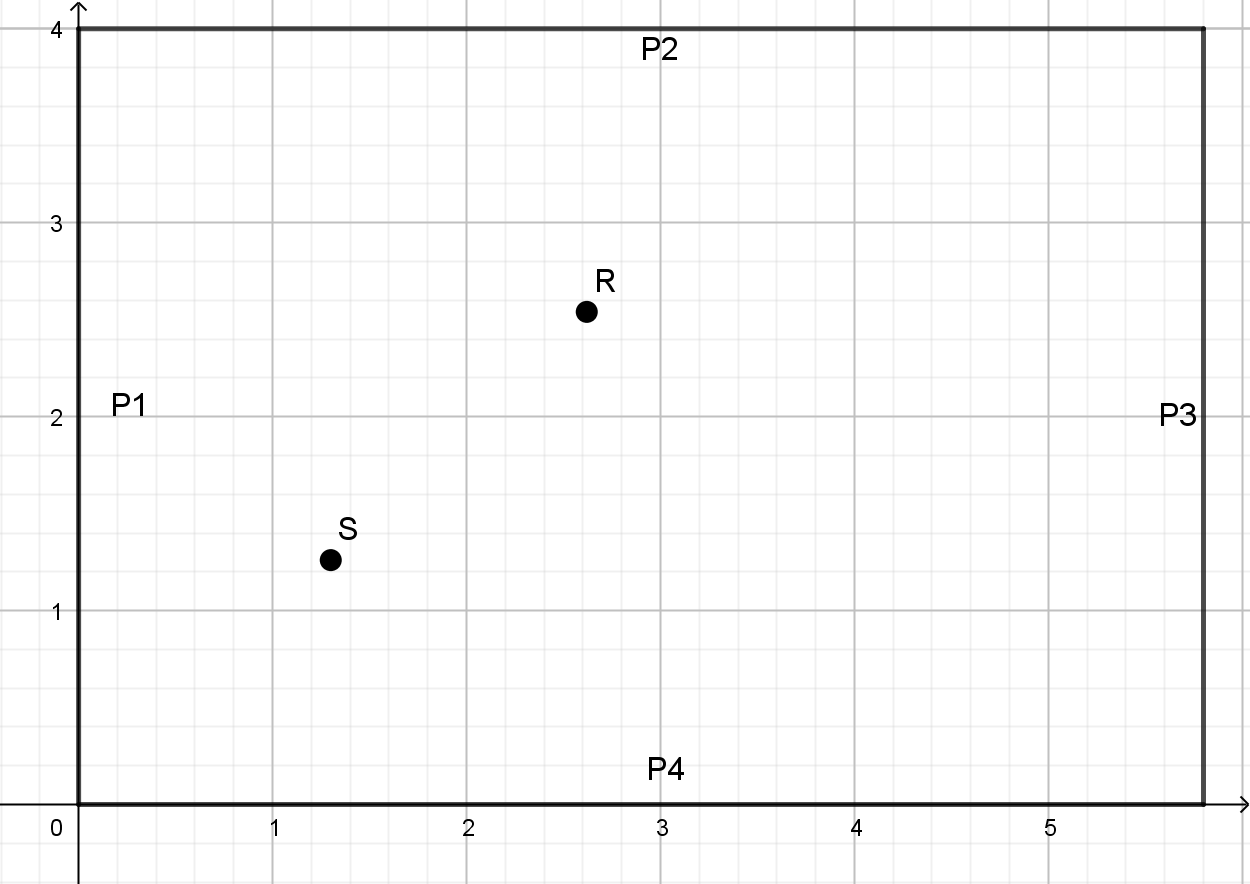
\includegraphics[width=12cm]{rys1}
	\caption{Model geometrii pomieszczenia (S - punkt źródła dźwięku, R - punkt obserwacji, Pn - kolejne powierzchnie odbijające).}
\end{figure}

Do znalezienia wszystkich źródeł pozornych N-tego rzędu należy wygenerować wszystkie $K^N$ wariacje z powtórzeniami zbioru $P$. Na wstępie możemy pominąć wariacje, w~których ta sama powierzchnia jest przynajmniej dwoma kolejnymi elementami ciągu, ponieważ promień dźwiękowy nie może dwukrotnie z rzędu odbić się od tej samej powierzchni. Każda wariacja reprezentuje jeden promień dźwiękowy, który odbija się kolejno od każdej powierzchni w~wariacji. Aby znaleźć źródło pozorne dla danego promienia dźwiękowego, należy odbić punkt źródła symetrycznie względem każdej z płaszczyzn w~wariacji (Rys. 2.2.). 

\begin{figure}[H]
        \centering
                \centering
                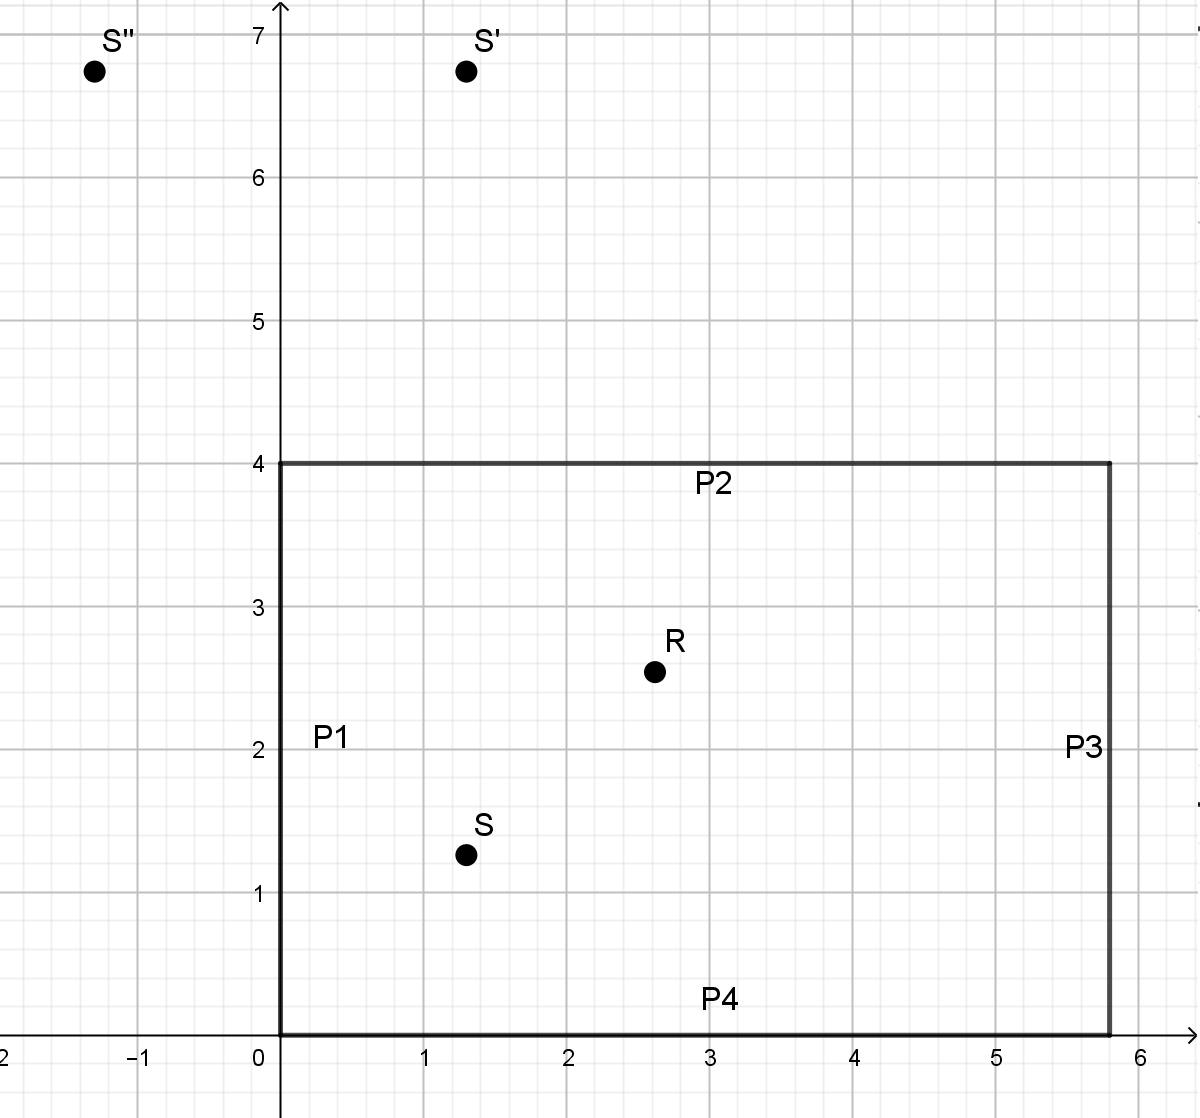
\includegraphics[width=12cm]{rys2}
	\caption{Pierwsze i~drugie odbicie względem powierzchni  (S - punkt źródła dźwięku, S' i S'' - kolejne odbicia symetryczne punktu S względem powierzchni odbijających, R - punkt obserwacji, Pn - kolejne powierzchnie odbijające).}
\end{figure}

Dla uzyskanego punktu należy zweryfikować, czy promień dźwiękowy jest w~stanie dotrzeć od punktu źródła do punktu odbiornika w~danym układzie geometrycznym. W tym celu należy prześledzić ścieżkę promienia dźwiękowego wstecz – zaczynając od punktu obserwacji. Początkowy kierunek promienia znajduje się wyznaczając wektor rozpięty od punktu źródła pozornego do punktu obserwacji. Prosta przechodząca przez te punkty powinna przecinać ostatnią powierzchnię z wariacji. Kąt pomiędzy wektorem wyznaczającym kierunek ścieżki promienia dźwiękowego a~wektorem normalnym płaszczyzny, na której leży powierzchnia odbijająca, powinien być mniejszy niż 90 stopni. Odcinek łączący punkt obserwacji z punktem przecięcia powyższej prostej z powierzchnią odbijającą stanowi fragment ścieżki promienia dźwiękowego. Kolejny fragment ścieżki promienia dźwiękowego wyznacza się odbijając symetrycznie poprzedni odcinek względem kolejnej powierzchni odbijającej. Z każdym krokiem należy sprawdzić, czy odcinek ścieżki promienia dźwiękowego przecina płaszczyzny, względem których się odbija. Jeśli uda się prześledzić ścieżkę promienia dźwiękowego od punktu obserwacji do punktu źródła, można sprawdzany punkt uznać za źródło pozorne i~uwzględnić w~siatce źródeł pozornych.

%---------------------------------------------------------------------------

\section{Uwzględnienie współczynnika pochłaniania}\label{sec:zm}

W akustyce architektonicznej, przy symulacji warunków akustycznych w~pomieszczeniu, istotne jest uwzględnienie współczynnika pochłaniania dźwięku (Wzór 2.1.). \\

\begin{equation}
\alpha=\frac{E_{poch}}{E_{pad}}
\end{equation}
gdzie
\begin{eqwhere}[2cm]
        \item[$E_{poch}$] energia fali pochłoniętej
        \item[$E_{pad}$] energia fali padającej
\end{eqwhere}

Definiując dla każdej powierzchni odbijającej współczynnik pochłaniania $\alpha_i$, gdzie $i$  jest indeksem powierzchni, możemy dla każdej z nich wyznaczyć współczynnik odbicia $R_i$. Mnożąc przez siebie współczynniki odbić fali dla kolejnych powierzchni i~przemnażając przez energię źródła otrzymujemy energię źródła pozornego odpowiadającego odbiciom od powyższych powierzchni (Wzór 2.2). \\

\begin{equation}
E_{IS}=E_{S}\cdot\prod_{i=1}^{N}(1-\alpha_i)
\end{equation}
gdzie
\begin{eqwhere}[2cm]
        \item[$E_{S}$] energia źródła dźwięku
        \item[$N$] liczba powierzchni odbijających
        \item[$\alpha_i$] współczynniki pochłaniania kolejnych powierzchni odbijających
\end{eqwhere}

%---------------------------------------------------------------------------

\section{Przykładowe użycie metody}\label{sec:przyuzy}

Przyjmując prostopadłościenne pomieszczenie z umieszczonym punktowym źródłem dźwięku i~punktem obserwacji (Rys. 2.3.), wyznaczamy siatkę źródeł pozornych (Rys. 3.4.). Dla przejrzystości rysunku siatka została wyznaczona dla maksymalnie trzeciego odbicia.
 
\begin{figure}[H]
        \centering
                \centering
                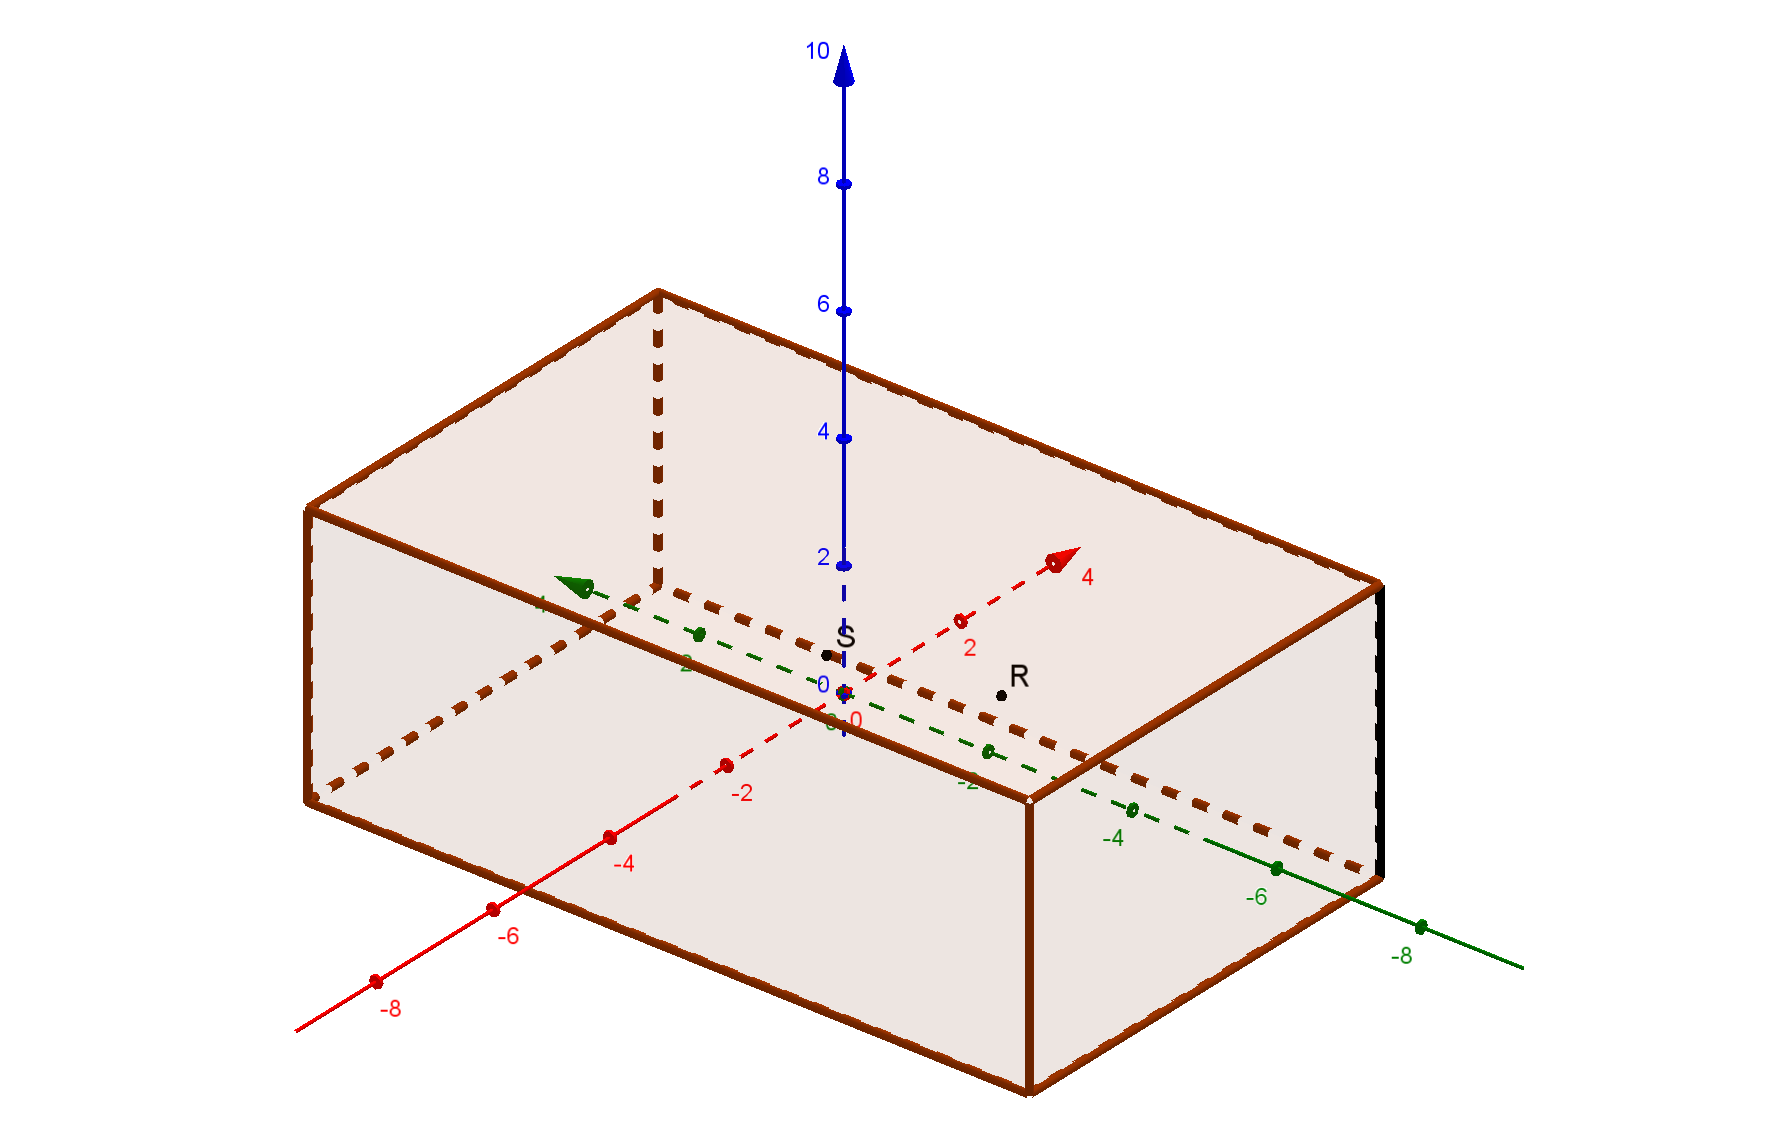
\includegraphics[width=12cm]{rys3}
	\caption{Model geometrii pomieszczenia (S - punkt źródła dźwięku, R - punkt obserwacji).}
\end{figure}

\begin{figure}[H]
        \centering
                \centering
                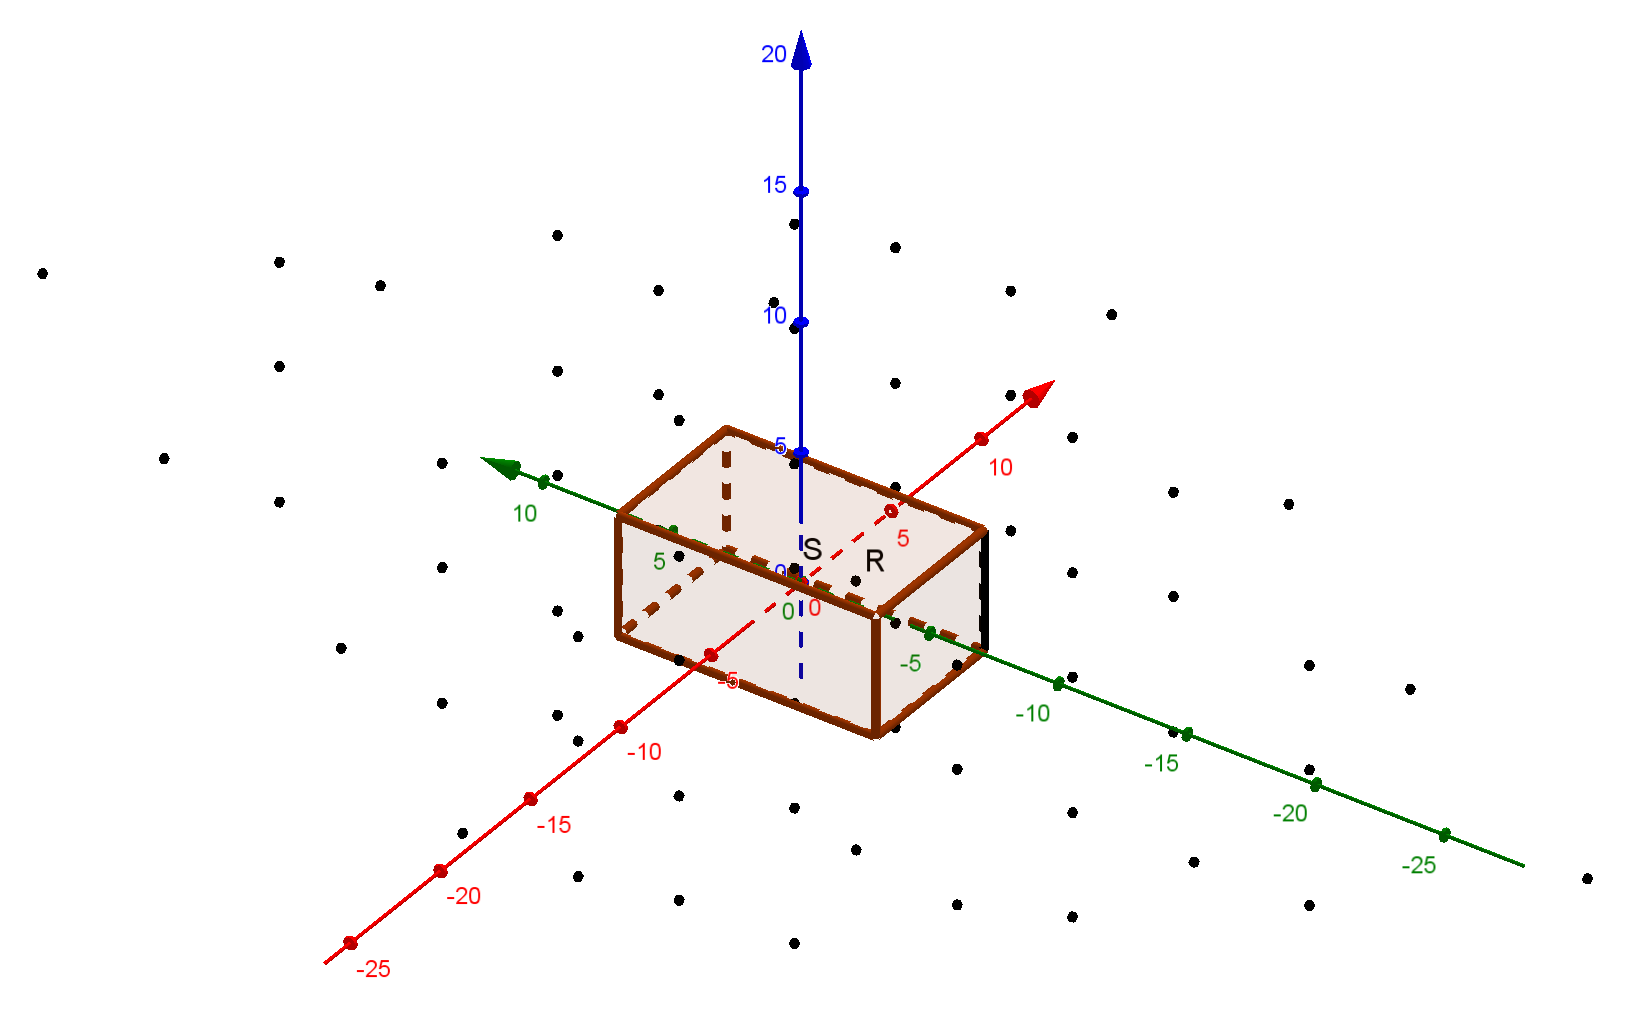
\includegraphics[width=12cm]{rys4}
	\caption{Siatka źródeł pozornych (S - punkt źródła dźwięku, R - punkt obserwacji).}
\end{figure}

Położenia  źródeł pozornych w~siatce dają informację o kierunkach promieni dźwiękowych dochodzących do punktu obserwacji. Uwzględniając straty energii pochłoniętej przez odbicia oraz starty energii związanej z rozchodzeniem się fali kulistej, możemy wyznaczyć  ilość energii i~czas, w~jakim dotrze ona do punktu obserwacji dla każdego źródła pozornego. Zależność energii dochodzącej do punktu odbioru od czasu przedstawiona jest na poniższym echogramie (Rys. 2.5.).

\begin{figure}[H]
        \centering
                \centering
                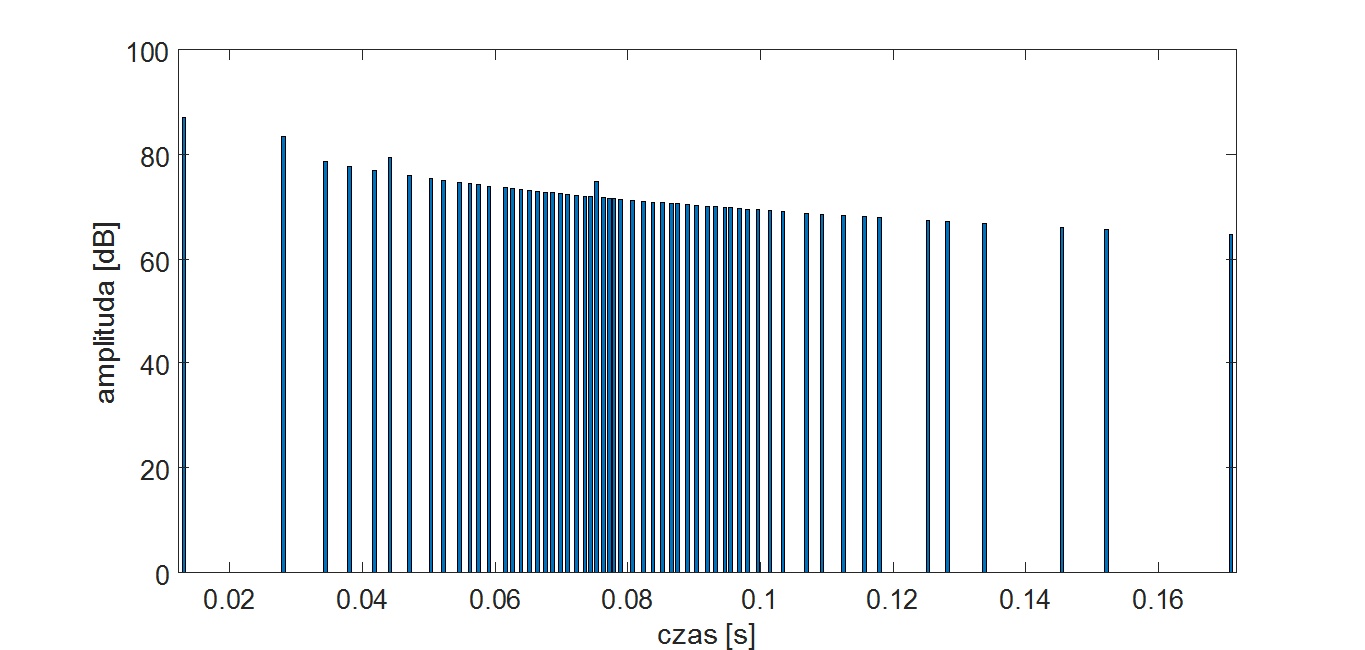
\includegraphics[width=16cm]{rys5}
	\caption{Echogram.}
\end{figure}

Uzyskany echogram lub jego część mogą być użyte do obliczenia wskaźników C50, C80, D50. Poprzez całkowanie wsteczne echogramu można uzyskać krzywą zaniku energii dźwięku w~pomieszczeniu (Rys. 2.6.).

\begin{figure}[H]
        \centering
                \centering
                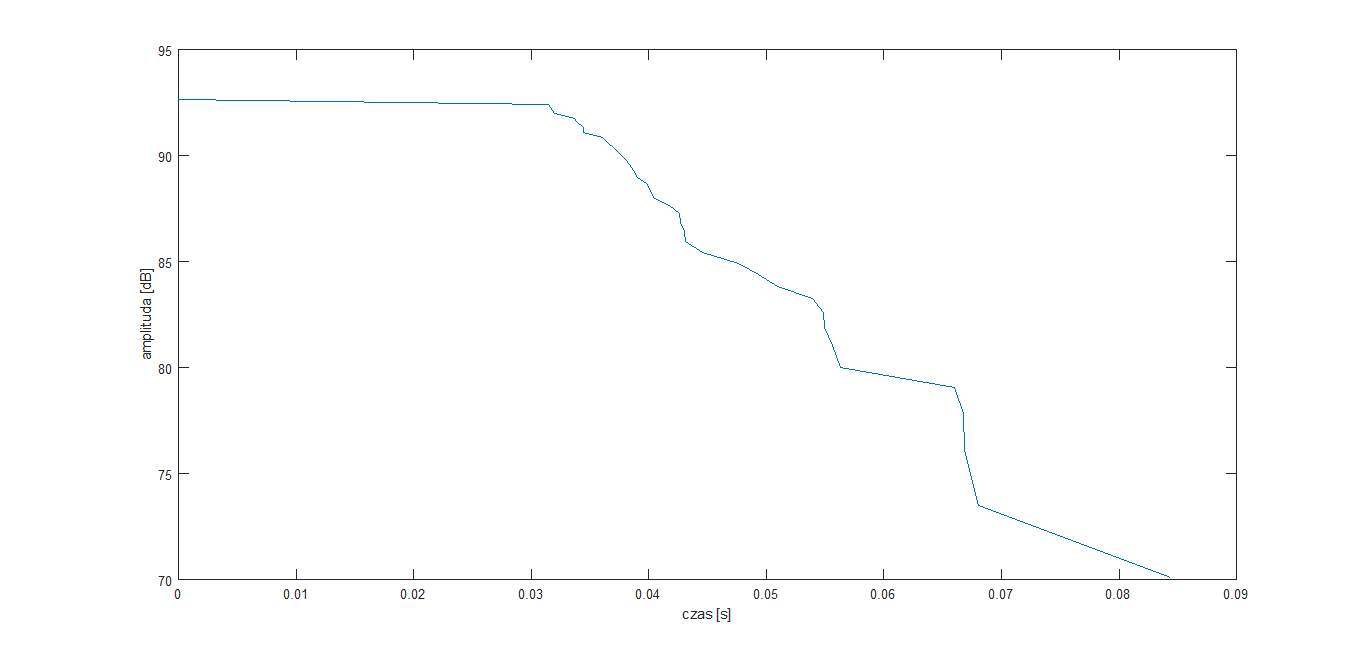
\includegraphics[width=16cm]{rys6}
	\caption{Krzywa zaniku dźwięku.}
\end{figure}

Na jej podstawie można wyznaczyć czas pogłosu pomieszczenia. W porównaniu do metody źródeł pozornych, w~metodzie promieniowej, ze względu na mniejszą złożoność obliczeń, uzyskuje się dłuższe echogramy. Zaletą metody źródeł pozornych jest uzyskiwanie dokładnych ścieżek promieni dźwiękowych, a~nie, jak w~przypadku metody promieniowej, ścieżek trafiających jedynie w~okolice punktu obserwacji. Ze względu na zalety obu tych metod często stosuje się je łącznie~\cite{b13}~\cite{b14}.
















\chapter{Przetwarzanie heterogeniczne}\label{cha:hpo}

%---------------------------------------------------------------------------

\section{Wprowadzenie}\label{sec:wprowadzenie}


Lata 50-te XX wieku były przełomowym okresem w dziedzinie elektronicznego przetwarzania danych. Opracowana w 1945 roku Architekura von Neumana [16] pozwoliła na uruchomienie pierwszych komputerów ogólnego przeznaczenia. Mimo, że Architektura Harwardzka [17] została opracowana 6 lat wcześniej, Architektura von Neumana była łatwiejsza w implementacji przez przechowywanie danych wraz z programem na jednej wspólnej pamięci. Pierwszym komputerem opartym na pomyśle Neumana, który wykonywał instrukcje zapisane w fizycznej pamięci , był powstały w 1948 roku Small-Scale Experimental Machine. Był on bazą do rozwijania kolejnych urządzeń i tak w 1949 roku powstał EDSAC (akronim od ang. Electronic Delay Storage Automatic Calculator). Został uznany jako  pierwszy komputer wykorzystywany w praktyce do obliczeń naukowych. EDSAC rozbudowany był o dodatkowe układy peryferyjne. W celu odczytu danych zastosowano w nim dalekopis – aparat drukujący dane w postaci alfanumerycznej. Skonstruowanie komputerów zerowej, pierwszej i drugiej generacji znacznie rozwinęło moc obliczeniową tych urządzeń. W dalszym ciągu jednak stosowano niewygodne formy prezentacji danych – wyświetlacze złożone z szeregu lamp, perforowane karty. W 1975 roku, w jednym z pierwszych komputerów osobistych IBM 5100, zastosowano kineskopowy wyświetlacz, który mógł wyświetlać 16 linii po 64 znaków. 6 lat później , w kolejnym modelu IBM 5150, wprowadzono możliwość instalacji kart rozszerzeń ISA. Zastosowano w nim pierwszą kartę graficzną Monochrome Display Adapter (MDA). Rozpoczęło to rozwój peryferyjnych układów komputera, które stały się niezależnymi platformami z własnym procesorem i pamięcią. Początkowo karty graficzne były w stanie wyświetlać jedynie znaki alfanumeryczne przechowywane w pamięci karty. Kolejne generacje kart pozwalały na rysowanie obrazów przy użyciu pojedynczych pikseli, a nowoczesne układy graficzne pozwalały na akcelerację 2D i 3D, korzystając z wbudowanych funkcji do generowania obrazu. W najnowszych procesorach grafiki umożliwiono użytkownikowi zaprogramowanie ich w dowolny sposób. Charakterystyka obliczeń przy przetwarzaniu obrazów wymusiła architekturę procesorów graficznych w postaci dużej ilości jednakowych jednostek ALU (ang. Arithmetic Logic Units), potrafiących wykonać równolegle wiele prostych operacji (Rys. 3.1.).
\begin{figure}[h]
        \centering
                \centering
                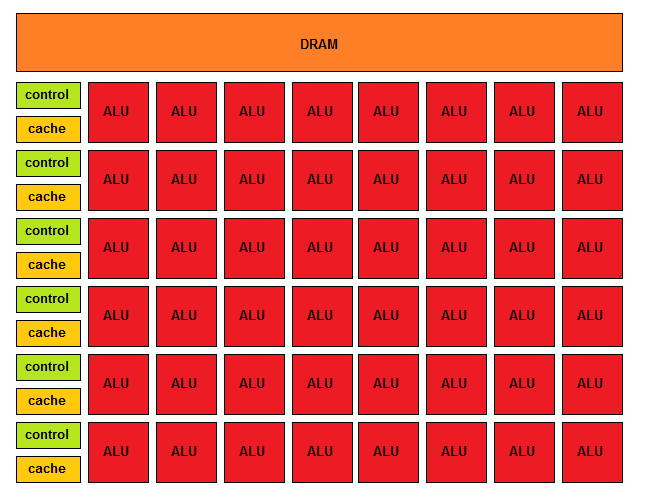
\includegraphics[width=12cm]{rys7}
	\caption{Architektura procesora GPU.}
\end{figure}
Taka budowa kart graficznych pozwoliła na wykorzystanie ich nie tylko do obliczeń związanych z generowaniem grafiki, ale także innych obliczeń przetwarzania danych , co doprowadziło do powstania kart ogólnego przeznaczenia (GPGPU).



%---------------------------------------------------------------------------

\section{Heterogeniczne platformy obliczeniowe}\label{sec:hetero}

Początkowo GPGPU były wykorzystywane do zaawansowanego generowania grafiki. Dążenie do realizmu w grach komputerowych rozwinęło karty graficzne o algorytmy wymagające przetwarzania równoległego, takie jak shading [18] czy ray-tracing [19]. W celu odciążenia procesora od złożonych obliczeń, na kartach graficznych zaczęto implementować fizykę obiektów – obliczenia związane z mechaniką klasyczną, symulacje zachowania cieczy, zachowania układów ciągłych i inne efekty cząsteczkowe. Dla ułatwienia programistom wykorzystania możliwości GPGPU, NVIDIA w 2007 roku wprowadza platformę CUDA. Jest to środowisko programistyczne i biblioteka umożliwiająca wykorzystanie kart graficznych produkowanych przez firmę NVIDIA. Umożliwia ona pisanie kodu opartego na C/C++ wykonywanego na procesorze karty i mającego bezpośredni dostęp do jej pamięci. Ułatwienie implementacji algorytmów na GPGPU rozwinęło wykorzystywanie tych kart w różnych dziedzinach naukowych, takich jak kryptografia, fizyka kwantowa, ekonomia czy medycyna. Wykonywanie  skomplikowanych obliczeń przy użyciu CUDA stało się powszechne na komputerach domowych, ale było ograniczone przez wymagania sprzętowe. 2 lata po wprowadzeniu CUDA firma Apple Inc wprowadza OpenCL (ang. Open Computing Language). W przeciwieństwie do produktu NVIDA, OpenCL umożliwia pisanie programów na heterogeniczne platformy – układy złożone z różnego rodzaju procesorów. Daje to możliwość pisania aplikacji na komputery z układami większości popularnych producentów, lub dowolne układy złożone z różnych procesorów (m. in. CPU, GPU, DSP, FPGA), oraz zapewnia przenośność programów.

%---------------------------------------------------------------------------

\section{Modele obliczeń równoległych}\label{sec:Paralellism}

Obliczenia równoległe to typ obliczeń komputerowych, w których wiele instrukcji wykonywanych jest jednocześnie [Gottlieb, Allan; Almasi, George S. (1989). Highly parallel computing. Redwood City, Calif.: Benjamin/Cummings. ISBN 978-0-8053-0177-9.]. Złożone problemy często mogą być rozłożone na mniejsze zadania, które mogą być wykonywane w tym samym czasie. Daje to możliwość szybszego rozwiązywania problemów bez zwiększania częstotliwości taktowania procesora. W uproszczeniu energia wydzielana przez procesor, a w większości ciepło, wzrasta wraz z kwadratem częstotliwości taktowania. Ze względu na te fizyczne ograniczenia procesora wielordzeniowe procesory i obliczenia równoległe stały się dominującym paradygmatem architektury komputerów.

Obliczenia równoległe dzielą się na cztery różne modele:

- równoległość bitów

- równoległość instrukcji

- równoległość danych

- równoległość zadań.

Modele obliczeń równoległych mogą być implementowane oddzielnie, lub w połączeniu ze sobą.

\subsection{Równoległość bitów}\label{sec:bitp}

Równoległość na poziomie bitów jest modelem przetwarzania równoległego opartym na zwiększaniu ilości bitów w pojedyńczym słowie procesora. Zwiększenie pojemności słowa zmniejsza liczbę instrukcji, które procesor musi wykonać, aby wykonać operację na zmiennych, których rozmiary są większe niż długość słowa.
Początkowo komputery opierały się na jednobitowych procesorach. Pierwszym nieszeregowym komputerem był 16-bitowy Whirlwind z 1951 roku. Obecnie w komputerach osobistych funkcjonuje standard 32 i 64-bitowych architektur procesorów i systemów operacyjnych. Większa szerokość słowa wymagałaby znacznie większej zewnętrznej szyny danych, co jest kosztowne do wykonania przy obecnych procesach technologicznych. 64-bitowe słowo w większości jest wystarczające do  procesowania zmiennych wykorzystywanych na komputerach osobistych. Przy złożonych obliczeniach inżynierskich duże dane przechowuje się na kilku zmiennych i przetwarza przy użyciu kilku instrukcji procesora.

\subsection{Równoległość instrukcji}\label{sec:instp}

Równoległość na poziomie instrukcji jest oparta na równoległym wykorzystaniu kilku jednostek wykonawczych procesora. Większość procesorów składa się z kilku jednostek arytmetyczno-logicznych ALU, odpowiadających za wykonywanie operacji arytmetycznych i logicznych przez procesor, oraz kilku jednostek zmiennoprzecinkowych FPU, odpowiadających za wykonywanie operacji arytmetycznych na liczbach zmiennoprzecinkowych. Wszystkie jednostki ALU i FPU mogą wykonywać operacje równolegle. Przykładowo, w poniższym kodzie (Kod ...), operacja z linijki 4 może być wykonana na jednostce ALU, a operacja z linijki 5 na jednostce FPU. Wykorzystując równoległość na poziomie instrukcji obie operacje mogą być wykonane przy użyciu jednej instrukcji procesora.

\begin{program}
\caption{Plik wejściowy programu}
\begin{lstlisting}
float a = 1.0, b = 2.0, c;
int x = 1, y = 2, z, w;

c = a + b;
z = z * y;
\end{lstlisting}
\end{program}

W zależności od architektury komputera, rozdzielenie operacji na jednostki wykonawcze procesora może być wykonane dynamicznie w trakcie wykonywania programu, lub statycznie na poziomie kompilacji. Dynamicznie ustawiana równoległość instrukcji wykorzystywana jest w powszechnie dostępnych procesorach CPU. Zwiększa ona szybkość wykonywania programu i odciąża programistę i kompilator od procesu rozdzielenia instrukcji. Rozmieszczenie instrukcji na etapie kompilacji wykorzystywane jest w procesorach DSP i GPU. Pozwala to optymalizację kodu przed jego wykonaniem i obliczenie dokładnego czasu w jakim program będzie się wykonywał.  

\subsection{Równoległość danych}\label{sec:datap}

Równoległość na poziomie danych wykorzystywana jest przy obliczeniach na dużych zbiorach danych, gdzie obliczenia dla pojedyńczych danych są od siebie niezależne. W tym modelu zbiór danych dzielony jest na mniejsze zbiory i definiowany jest zestaw zadań, które zostaną wykonane na pojedyńczego zbioru. Mniejsze zbiory danych wysyłane są do oddzielnych jednostek sterujących, które wykonują na nich równolegle zdefinowany zestaw zadań. Równoległość danych jest najwydajniejsza dla dużych zbiorów podobnych danych (np. wektory, macierze), dla prostych operacji, takich mnożenie macierzy, transformata Fouriera. Szybkość wykonywania programu opartego na tym modelu zależy od ilości jednostek sterujących, dlatego paralelizm danych często implementowany jest na procesorach graficznych, gdzie ilość tych jednostek sięga kilku tysięcy.

\subsection{Równoległość zadań}\label{sec:taskp}

Równoległość na poziomie zadań to model gdzie równolegle wykonywane są różne zadania na tych samych, lub różnych zbiorach danych. Najczęściej wykorzystywany jest na wielordzeniowych procesorach CPU, gdzie każdy rdzeń może wykonywać bardziej złożone operacji niż w przypadku modelu równoległości danych. Rozdzielenie zadań pomiędzy rdzenie wykonywany jest na poziomie pisania kodu aplikacji, lub obsługiwane przez system operacyjny. Większość współczesnych systemów operacyjnych wykorzystuje równoległość zadań do wykonywania procesów na oddzielnych wątkach.

%---------------------------------------------------------------------------

\section{Środowisko OpenCL}\label{sec:OpenCL}

OpenCL jest platformą programistyczną opracowaną w 2009 roku przez Apple Inc, a następnie utrzymywaną przez Khronos Group. Umożliwia programowanie heterogenicznych układów procesorowych w języku opartym na C99 i C++11. Wykorzystanie OpenCL nie ogranicza się jedynie do procesorów graficznych. Jego głowną zaletą jest przenośność na większość popularnych procesorów CPU, DSP, a nawet układów FPGA. Każdy procesor z instrukcjami SSE2 może zostać wykorzystany jako urządzenie OpenCL. Standard OpenCL dostarcza interfejs programistyczny (API), biblioteki dla wielu popularnych języków programowania oraz sterowniki do urządzeń.

\subsection{Platforma}\label{sec:platforma}

Aplikacja pisana w OpenCL opiera się na jednostkach zwanych platformami. Każda platforma odpowiada za przygotowanie danych do obliczeń i rozdzielenie zadań. W nowszych standardach kod platformy może być pisany w wielu popularnych językach  (m. in. Python, Matlab). Każda platforma zawiera kontekst, w którym definiowane są dane wejściowe, kolejka zadań i urządzenia do wykonywania obliczeń. Każde urządzenie zawiera jednostki obliczeniowe (ang. compute units, CU), które składają się z elementów przetwarzania (ang. processing elements, PEs)(Rys. 3.2.). 

\begin{figure}[h]
        \centering
                \centering
                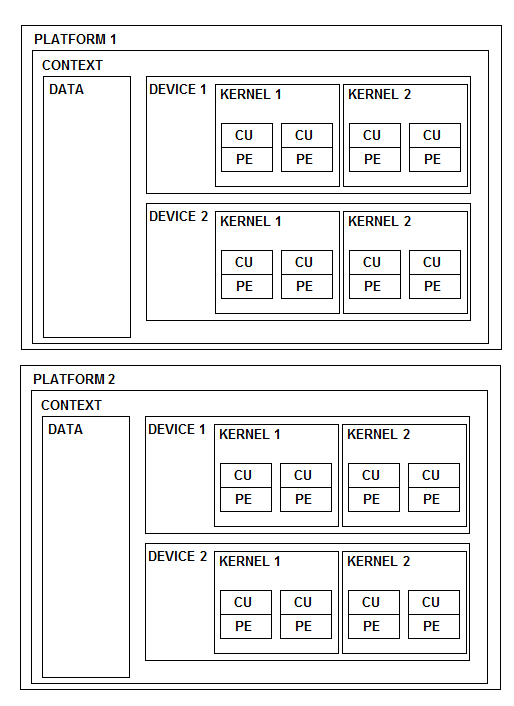
\includegraphics[width=12cm]{rys8}
	\caption{Architektura programu napisanego w bibliotece OpenCL.}
\end{figure}

Pojedyńcza platforma odnosi się do poszczególnego sterownika. Przykładowo na komputerze z procesorem Intel i kartą graficzną AMD mozemy uruchomić dwie platformy, jedną dla OpenCL™ Runtimes for Intel® Processors [https://software.intel.com/en-us/articles/opencl-drivers] i drugą dla wyspecjalizowanego sterownika AMD dla danej karty graficznej. Każda platforma może obsługiwać więcej niż jedno urządzenie, w szczególnych przypadkach może zawierać złożone układy kart graficznych.

\subsection{Urzadzenia OpenCL}\label{sec:OpenC21L}

Standard OpenCL udostępnia 5 różnych rodzajów urządzeń:

- CL_DEVICE_TYPE_CPU - 

\subsection{Kontekst obliczeniowy}\label{sec:OpenC2L}


\subsection{Jednostki obliczeniowe i elementy przetwarzania}\label{sec:OpenC3L}
\subsection{Kernel}\label{sec:OpenC4L}
\subsection{Przestrzen indeksowania}\label{sec:OpenC5L}
Jednostki obliczeniowe i elementy przetwarzania reprezentują różne fizyczne elementy procesora w zależności od jego rodzaju. Dla procesorów CPU CU jest równoważne PE i stanowi pojedyńczy rdzeń procesora. W kartach graficznych NVIDIA CU stanowi multiprocesor strumieniowy, a PE jego rdzenie. Karty graficzne AMD definiują CU jako jednostkę SIMD (ang. Single instruction, multiple thread), a PE jako poszczególne linie jednostki SIMD. Elementy przetwarzania wykonują specjalnie przygotowane funkcje (tzw. kernele), definiowane według standardu OpenCL. Mimo że w zależności od urządzenia CU i PE reprezentują różne elementy procesora, odwołują się do nich w ten sam sposób. Umożliwia to wykonywanie  kernela o jednakowej składni na różnych typach procesorów. Kernele wykonywane są według kolejki zadań i rozdzielone pomiędzy jednostki obliczeniowe mogą być wykonywane równolegle na wielu elementach przetwarzania. Każda kolejka zadań definiuje przestrzeń indeksowania, w której wykonywane są poszczególne kernele.  Instancje kernela wywołaną w obrębie jednego indeksu nazywamy wątkiem. Przestrzeń indeksów można podzielić na grupy (ang. work-group), do których należą poszczególne wątki.

\subsection{Dostep do pamieci}\label{sec:OpenC6L}

OpenCL umożliwia dynamiczny dostęp do pamięci urządzeń. Zdefiniowane są cztery typy pamięci:

- pamięć globalna – pamięć dostępna przez wszystkie wątki w obrębie jednego kontekstu

- pamięć stała – pamięć tylko do odczytu, dostępna globalnie

- pamięć lokalna – pamięć dostępna w obrębie jednej grupy wątków

- pamięć prywatna – pamięć dostępna w obrębie jednego wątku\\


 Przepływ danych między platformą  a urządzeniem może odbyć się poprzez operację kopiowania  lub odwzorowania z pamięci platformy do pamięci urządzenia.

Dużym ograniczeniem wydajności obliczeń jest czas dostępu do pamięci. Pamięć o szerszym zakresie ma wolniejszy czas dostępu, dlatego najwydajniejsze obliczeniawykonują się dla niezależnych wątków działających równolegle o prywatnej pamięci.
















\chapter{Realizacja założeń projektowych}\label{cha:rzp}

%---------------------------------------------------------------------------

\section{Wprowadzenie}\label{sec:wprowadzenie}


Promowany w latach 80-tych ruch wolnego oprogramowania [20] znacząco wpłynął na rozwój aplikacji i algorytmów. Powszechny dostęp do Internetu umożliwił upublicznianie kodów źródłowych, co zrzeszało duże społeczności pracujące wspólnie nad rozwojem programów komputerowych. Otwarte bazy aplikacji i algorytmów pozwoliły niezależnym programistom  na wykorzystanie ich do rozwoju kolejnych w wydajniejszy sposób. Realizacja projektu niniejszej pracy stanowi bazę, która może zostać wykorzystana w podobny sposób. Kod tej aplikacji może być łatwo zaadaptowany do połączenia jej z innym oprogramowaniem. Możliwe też jest wprowadzenie modyfikacji algorytmu metody źródeł pozornych  lub zaimplementowanie dodatkowych metod wewnątrz aplikacji.


Aplikacja została napisana przy użyciu OpenCL w wersji 1.2. Zdecydowano się na starszą wersję ze względu na kompatybilność z wieloma popularnymi urządzeniami. Platforma została napisana przy użyciu języka C++11. Zarówno dane wejściowe jak i wyjściowe transferowane są między plikiem wykonywalnym a plikami tekstowymi.    



%---------------------------------------------------------------------------

\section{Implementacja algorytmu}\label{sec:ra}

Aplikacja do obliczeń używa jednej platformy (Kod źr. 1.), która definiuje jeden kontekst obliczeniowy i jedno urządzenie.
\begin{program}
\caption{Definiowanie platformy}
\begin{lstlisting}
cl_platform_id* platforms = new cl_platform_id[numPlatforms];
status = clGetPlatformIDs(numPlatforms, platforms, NULL);
\end{lstlisting}
\end{program}
Dane wejściowe alokowane są w pamięci po stronie platformy. Następnie tworzony jest kontekst obliczeniowy (Kod źr. 2.), który przy użyciu predyrektywy \verb|CL_PRESENT_DEVICE| wybiera , jaki typ urządzenia zostanie wybrany.
\begin{program}
\caption{Definiowanie kontekstu obliczeniowego}
\begin{lstlisting}
cl_context_properties cps[3] = { CL_CONTEXT_PLATFORM, (cl_context_properties)platform, 0 };
context = clCreateContextFromType(
                                  cps, 
                                  CL_PRESENT_DEVICE, 
                                  NULL, 
                                  NULL, 
                                  &status);
\end{lstlisting}
\end{program}
Następuje poszukiwanie urządzenia o zadanym typie i zapisanie informacji o nim (Kod źr. 3.).
\begin{program}
\caption{Pobieranie listy dostępnych urządzeń}
\begin{lstlisting}
clGetContextInfo(
                 context, 
                 CL_CONTEXT_DEVICES, 
                 deviceListSize, 
                 devices, 
                 NULL);

\end{lstlisting}
\end{program}
Kolejnym krokiem jest przygotowanie kolejki zadań (Kod źr. 4.). Posłuży ona do stworzenia przestrzeni indeksowania dla wątków.
\begin{program}
\caption{Przygotowanie kolejki zadań}
\begin{lstlisting}
commandQueue = clCreateCommandQueue(
                                    context, 
                                    devices[0], 
                                    0, 
                                    &status);
\end{lstlisting}
\end{program}
Dane wejściowe przekazywane są do kontekstu obliczeniowego poprzez bufory (Kod źr. 5.). Oddzielne bufory dla każdej danej wejściowej transferują owe  dane do zdefiniowanego przez kernel miejsca w pamięci. 
\begin{program}
\caption{Definicja buforu danych dla parametru plA}
\begin{lstlisting}

plABuffer = clCreateBuffer(
                           context, 
                           CL_MEM_READ_WRITE | CL_MEM_USE_HOST_PTR,
                           sizeof(cl_float) * walls,
                           plA, 
                           &status);
\end{lstlisting}
\end{program}
Kernel przechowywany jest w postaci pliku tekstowego (załącznik A). Plik ten jest wczytywany przez platformę, a następnie budowany do obiektu (Kod źr. 6.), który później będzie wywoływany przez poszczególne wątki. Kod kernela zawiera implementację metody źródeł pozornych na podstawie danych z kontekstu obliczeniowego. Ilość wszystkich wariacji powierzchni odbijających dla $N$ powierzchni i $L$ rzędu źródeł pozornych wynosi $N^L$. Przestrzeń indeksowania stanowi kolejne liczby od 1 do $N^L$. Dla każdego wątku indeks przedstawiany jest w postaci liczby w systemie liczbowym o podstawie N. Każda kolejna cyfra takiej liczby odpowiada poszczególnej płaszczyźnie, dzięki czemu dla każdego indeksu uzyskujemy unikatową wariację powierzchni odbijających.
\begin{program}
\caption{Budowanie obiektu kernela}
\begin{lstlisting}
program = clCreateProgramWithSource(
                                    context, 
                                    1, 
                                    &source,
                                    sourceSize,
                                    &status);
status = clBuildProgram(program, 1, devices, NULL, NULL, NULL);
kernel = clCreateKernel(program, "templateKernel", &status);
\end{lstlisting}
\end{program}
W zależności od wykorzystywanego urządzenia należy dobrać odpowiednio wielkości grup wątków. Zostały one zdefiniowane w zmiennych globalThreads i localThreads. Należy zwrócić uwagę , aby nie przekraczały one maksymalnych dopuszczalnych wartości dla danego urządzenia. W tym celu pobierane są informacje z bieżącego urządzenia o maksymalnych dopuszczalnych wartościach (Kod źr. 7.).
\begin{program}
\caption{Pobranie informacji o zasobach urządzenia}
\begin{lstlisting}
clGetDeviceInfo(
                devices[0], 
                CL_DEVICE_MAX_WORK_GROUP_SIZE, 
                sizeof(size_t), 
                (void*)&maxWorkGroupSize, 
                NULL);
clGetDeviceInfo(
                devices[0], 
                CL_DEVICE_MAX_WORK_ITEM_DIMENSIONS, 
                sizeof(cl_uint), 
                (void*)&maxDims, 
                NULL);
clGetDeviceInfo(
                devices[0], 
                CL_DEVICE_MAX_WORK_ITEM_SIZES, 
                sizeof(size_t)*maxDims,
                (void*)maxWorkItemSizes,
                NULL);
\end{lstlisting}
\end{program}
Przed uruchomieniem kernela przekazywany jest do niego bufor danych (Kod źr. 8.).
\begin{program}
\caption{Przekazanie bufora plABuffer do kernela}
\begin{lstlisting}

clSetKernelArg(
               kernel, 
               1, 
               sizeof(cl_mem), 
               (void *)&plABuffer);
\end{lstlisting}
\end{program}
Następuje uruchomienie kolejki zadań i czekanie na ich wykonanie (Kod źr. 9.). Po wykonaniu zadań kolejka zostaje zwolniona.
\begin{program}
\caption{Uruchomienie kolejki zadań dla bufora wejściowego}
\begin{lstlisting}
clEnqueueNDRangeKernel(
                       commandQueue,
                       kernel,
                       1,
                       NULL,
                       globalThreads,
                       localThreads,
                       0,
                       NULL,
                       &events[0]);
clWaitForEvents(1, &events[0]);
clReleaseEvent(events[0]);
\end{lstlisting}
\end{program}
Następnie dane wyjściowe odczytywane są z bufora wyjściowego (Kod źr. 10.)
\begin{program}
\caption{Uruchomienie kolejki zadań dla bufora wyjściowego}
\begin{lstlisting}
clEnqueueReadBuffer(
                    commandQueue,
                    outputBuffer,
                    CL_TRUE,
                    0,
                    width * sizeof(cl_uint),
                    output,
                    0,
                    NULL,
                    &events[1]);
\end{lstlisting}
\end{program}


%---------------------------------------------------------------------------

\section{Obsługa aplikacji}\label{sec:oa}

Przed kompilacją programu należy przygotować kod pod urządzenia , na jakich  będzie on wykonywany. W zależności od typu procesora należy zdefiniować dyrektywę \verb|CL_PRESENT_DEVICE| jako \verb|CL_DEVICE_TYPE_CPU| dla procesorów, lub \verb|CL_DEVICE_TYPE_GPU| dla kart graficznych. W zależności od parametrów urządzenia należy odpowiednio zdefiniować rozmiary grup wątków w zmiennych localThreads i globalThreads, a następne skompilować do pliku wykonywalnego dołączając biblioteki standardu OpenCL. Plik wykonywalny przyjmuje dane w postaci pliku wejściowego o nazwie input.txt. W danym pliku należy zdefiniować w kolejnych liniach  rząd pozornych źródeł, współrzędne punktu źródła dźwięku i punktu obserwacji, współczynniki płaszczyzn powierzchni odbijających w postaci ogólnej, granice powierzchni dla poszczególnych osi oraz współczynniki pochłaniania dźwięku dla każdej powierzchni (Kod źr. 11).

\begin{program}
\caption{Plik wejściowy programu}
\begin{lstlisting}
3              %rząd siatki źródeł pozornych
0.2, 0.4, 0.3  % współrzędne punktu źródła
0.6, -1.7, 0.4 % współrzędne punktu obserwacji
0, 0, 1, 3.3   % współczynniki płaszczyzny dla pierwszej powierzchni odbijającej 
-2, -7, -3.3   % dolne granice powierzchni dla osi x, y i z 
2, 7, -3.3     % gorne granice powierzchni dla osi x, y i z
0.71           % współczynnik pochłaniania powierzchni
\end{lstlisting}
\end{program}

Dane wyjściowe otrzymywane są w postaci pliku output.txt. Po wykonaniu obliczeń w pliku znajdują się współrzędne punktów siatki źródeł pozornych wraz z ich energią.

Przy ustawieniu dyrektywy \verb|write_file| na $true$ i wybraniu kombinacji powierzchni odbijających program wygeneruje plik ze skryptem wejściowym do programu GeoGebra. Wygenerowany skrypt rysuje trójwymiarową grafikę (Rys. 4.1.), na której znajdują się powierzchnie odbijające, punkt źródła dźwięku, punkt pozornego źródła, punkt obserwacji oraz ścieżka promienia dźwiękowego.
\begin{figure}[h]
        \centering
                \centering
                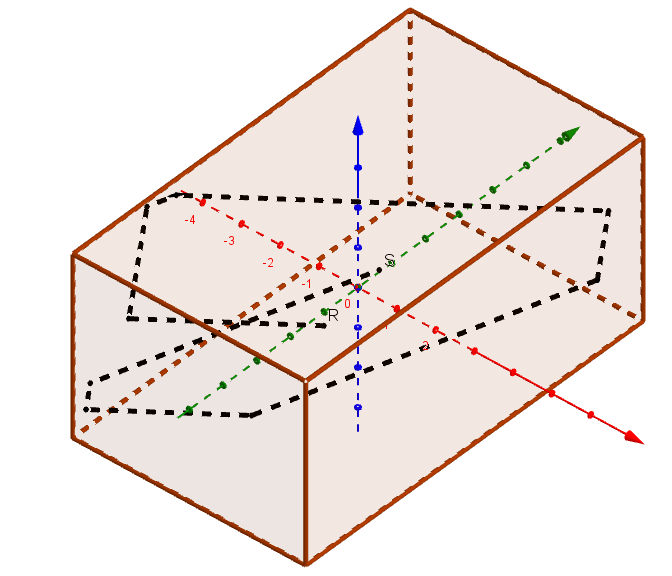
\includegraphics[width=12cm]{rys10}
	\caption{Ścieżka promienia dźwiękowego.}
\end{figure}
Dane z pliku output.txt mogą posłużyć do wygenerowania siatki źródeł pozornych (Rys. 4.2.).
\begin{figure}[h]
        \centering
                \centering
                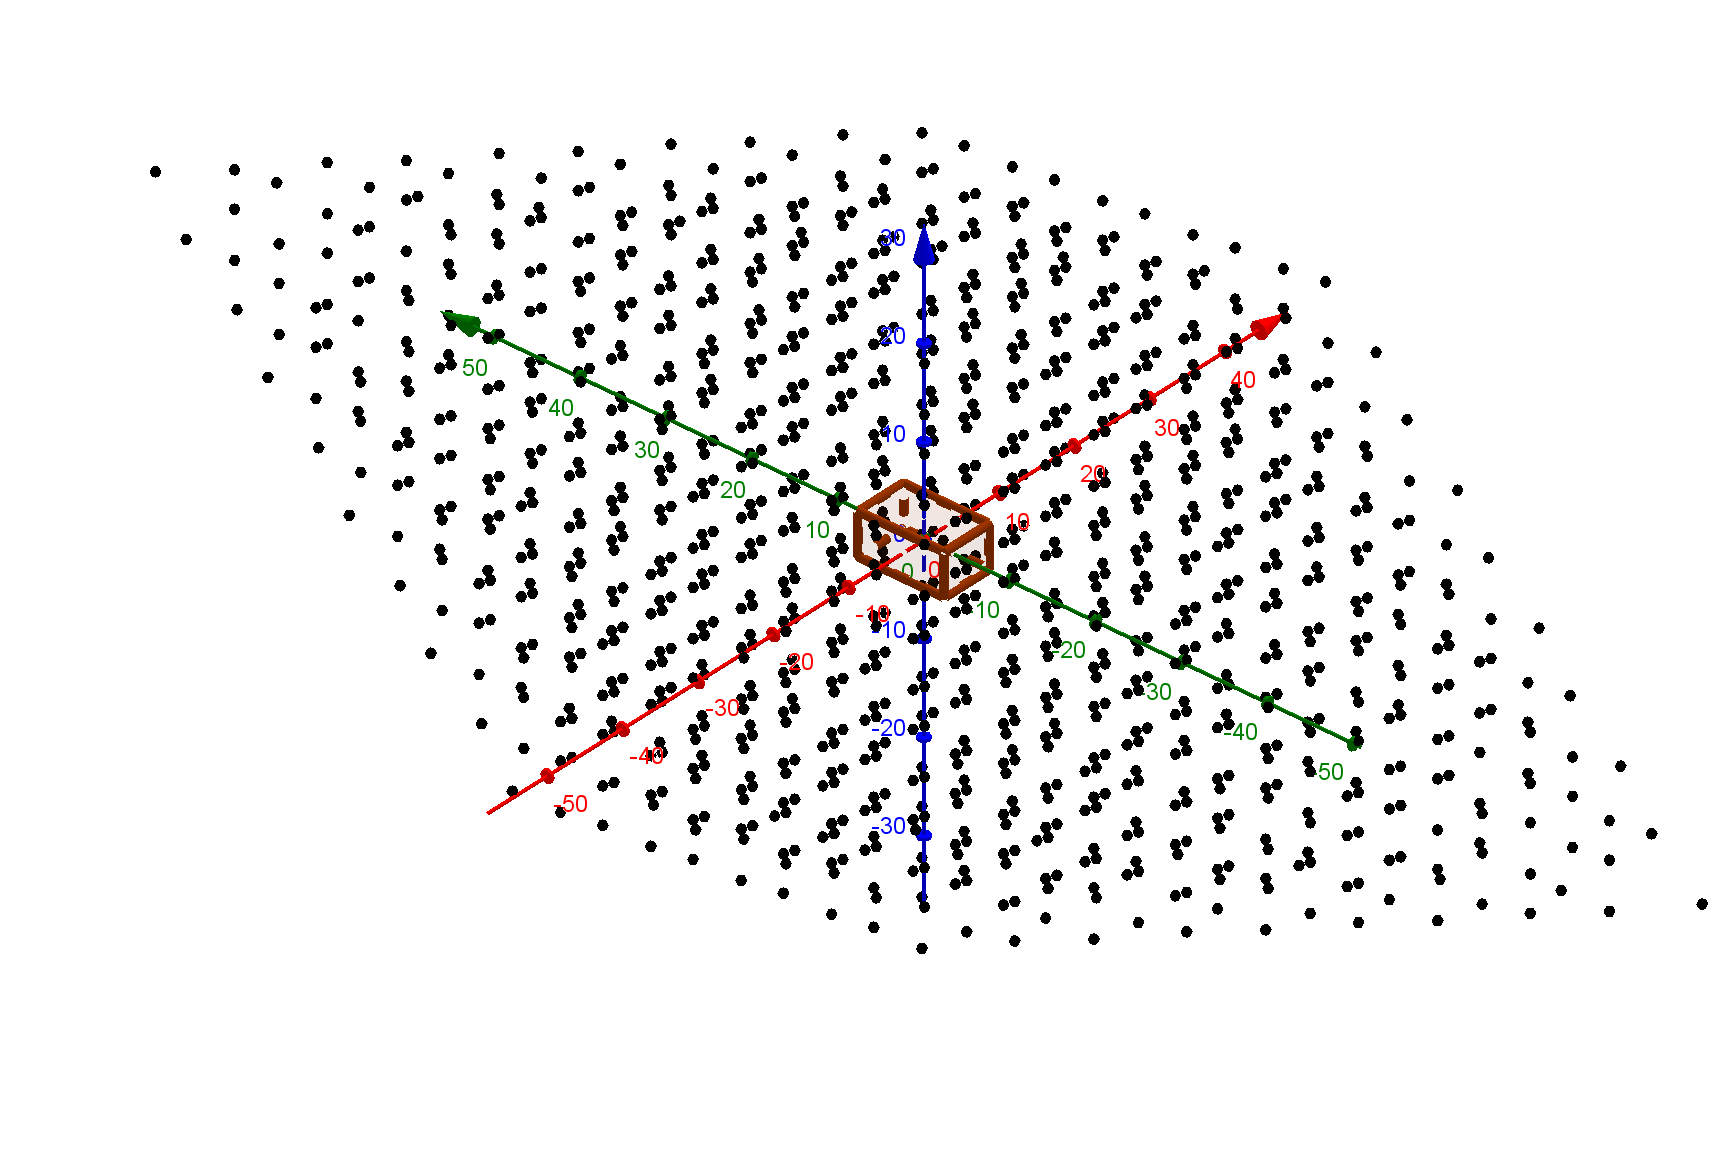
\includegraphics[width=12cm]{rys11}
	\caption{Siatka źródeł pozornych.}
\end{figure}














\chapter{Obliczenia testowe}\label{cha:ot}


%---------------------------------------------------------------------------

\section{Wprowadzenie}\label{sec:wprowadzenie}


Poza realizacją algorytmu autor wykonuje testy napisanej aplikacji. Testy poprawności implementacji zostały wykonane na podstawie testów jednostkowych. Przy użyciu ów testów autor sprawdza poprawność przekształceń geometrycznych i~transferu danych między pamięciami urządzeń. Test poprawności całego modelu wykonano wyznaczając algebraicznie siatki źródeł pozornych dla kilku początkowych rzędów dla różnych układów geometrycznych pomieszczeń i~porównując je z wynikami uzyskanymi przez obliczenia przy użyciu aplikacji. Testy dla źródeł pozornych wyższych rzędów zostały wykonane dla pojedynczych punktów.

W rozdziale 6.2 autor przedstawia przykładowe wykorzystanie aplikacji do analizy pola akustycznego. W tym celu przygotowane zostały geometryczne modele pomieszczeń o zróżnicowanych wymiarach i~parametrach pochłaniania dźwięku, a~następnie  porównane ze sobą. Aplikacja umożliwia jedynie obliczenia na bryłach wypukłych z powierzchniami prostopadłymi do osi układu współrzędnych. Ogranicza to model geometrii do prostopadłościanu z możliwością naniesienia dodatkowych powierzchni o innym współczynniku pochłaniania na ściany boczne tego prostopadłościanu.

W celu weryfikacji jednego z założeń pracy dotyczącego wydajności aplikacji autor uruchamia program na różnych urządzeniach. Do testów wykorzystane zostały urządzenia  zróżnicowane pod względem wydajności i~ilości jednostek arytmetyczno-logicznych. Autor porównuje czasy obliczeń na danych urządzeniach dla różnych rzędów siatki źródeł pozornych.

%---------------------------------------------------------------------------
\section{Użycie aplikacji}\label{sec:asdasd}

\subsection{Obliczenia na pomieszczeniach zróżnicowanych geometrycznie}\label{sec:imstest1}

Do obliczeń dla zróżnicowanych pomieszczeń zdefiniowano 3 modele geometryczne (Tabele 6.1-6.3).

\begin{table}[H]
        \centering
        \begin{threeparttable}
                \caption{Geometryczny model pomieszczenia 1}\label{tab:table_example}
                \begin{tabularx}{0.6\textwidth}{| c | X | X | X |}
                        \midrule
                        		&	x & y & z \\
		Wymiary pomieszczenia & 6 & 10 & 4.6 \\
                        Źródło & 0.2 & 0.4 & 0.33 \\
		Punkt obserwacji & 0.6 & -1.7 & 0.4 \\
                        \bottomrule
                \end{tabularx}
        \end{threeparttable}
\end{table}

\begin{table}[H]
        \centering
        \begin{threeparttable}
                \caption{Geometryczny model pomieszczenia 2}\label{tab:table_example}
                \begin{tabularx}{0.6\textwidth}{| c | X | X | X |}
                        \midrule
                        		&	x & y & z \\
		Wymiary pomieszczenia & 6 & 10 & 4.6 \\
                        Źródło & -2.9 & -4.9 & -2.2 \\
		Punkt obserwacji & -2.87 & -4.39 & -2.08 \\
                        \bottomrule
                \end{tabularx}
        \end{threeparttable}
\end{table}

\begin{table}[H]
        \centering
        \begin{threeparttable}
                \caption{Geometryczny model pomieszczenia 3}\label{tab:table_example}
                \begin{tabularx}{0.6\textwidth}{| c | X | X | X |}
                        \midrule
                        		&	x & y & z \\
		Wymiary pomieszczenia & 20 & 2 & 2 \\
                        Źródło & -9 & 0.2 & 0.3 \\
		Punkt obserwacji & 8 & -0.4 & 0.1 \\
                        \bottomrule
                \end{tabularx}
        \end{threeparttable}
\end{table}

Dla danych modeli zostały wykonane wyliczenia siatek źródeł pozornych do 12 rzędu (Rys. 6.1-6.3).

\begin{figure}[H]
        \centering
                \centering
                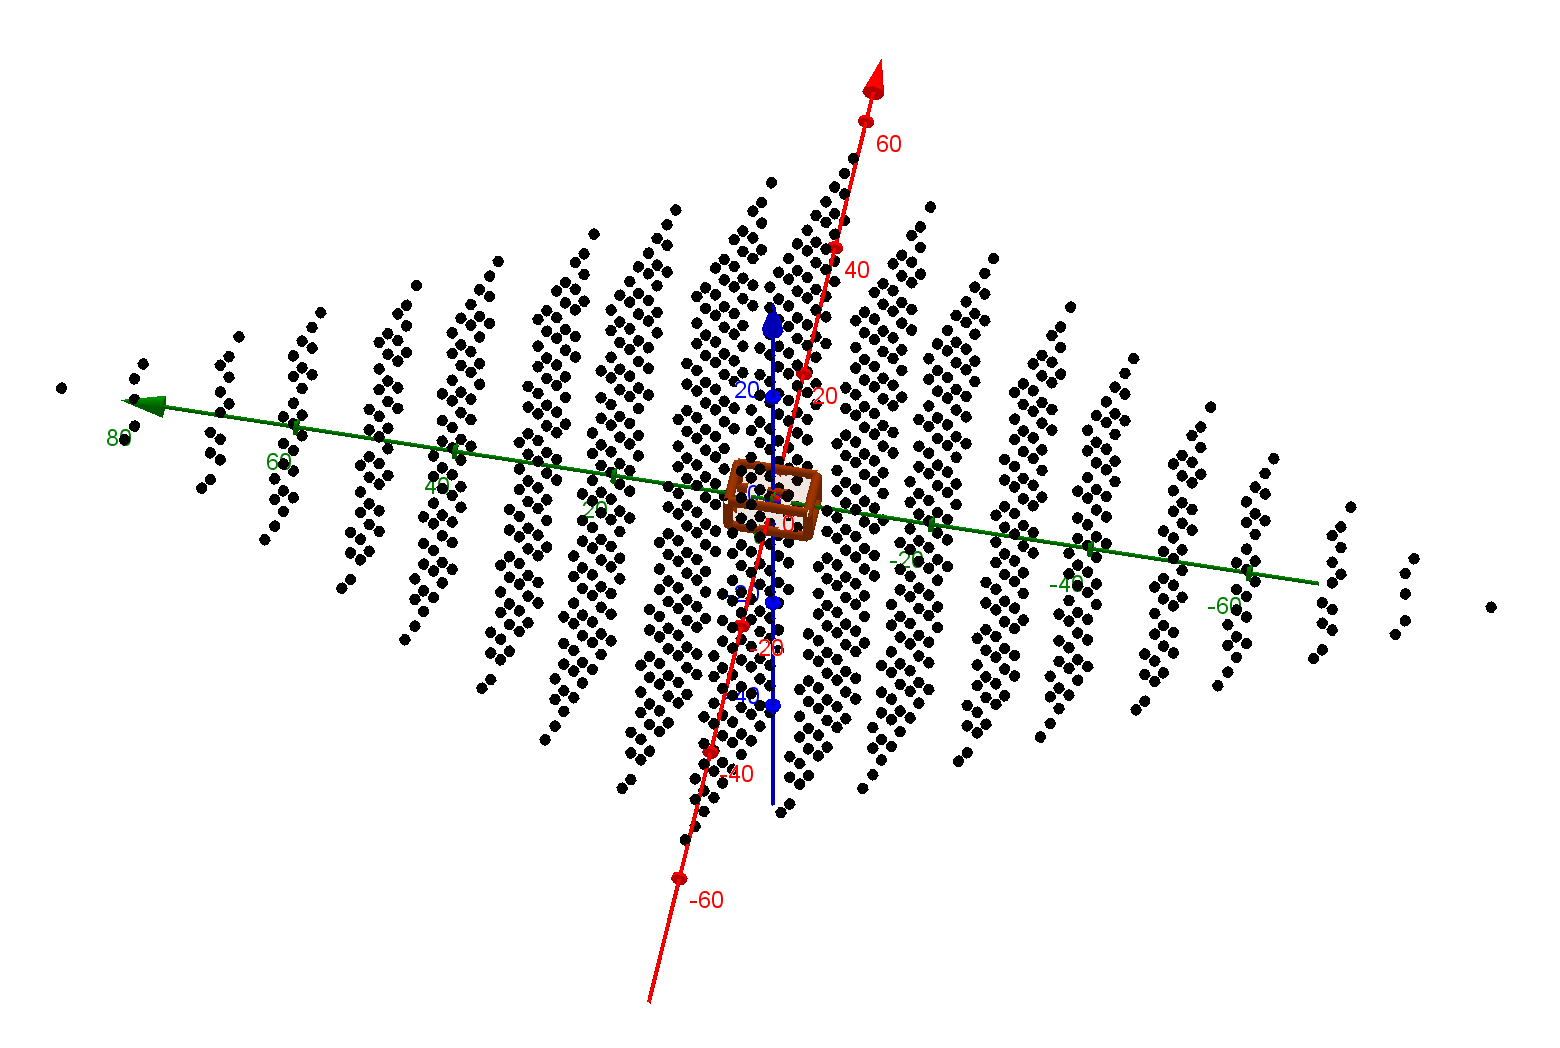
\includegraphics[width=12cm]{siatka1}
	\caption{Siatka źródeł pozornych modelu 1.}
\end{figure}

\begin{figure}[H]
        \centering
                \centering
                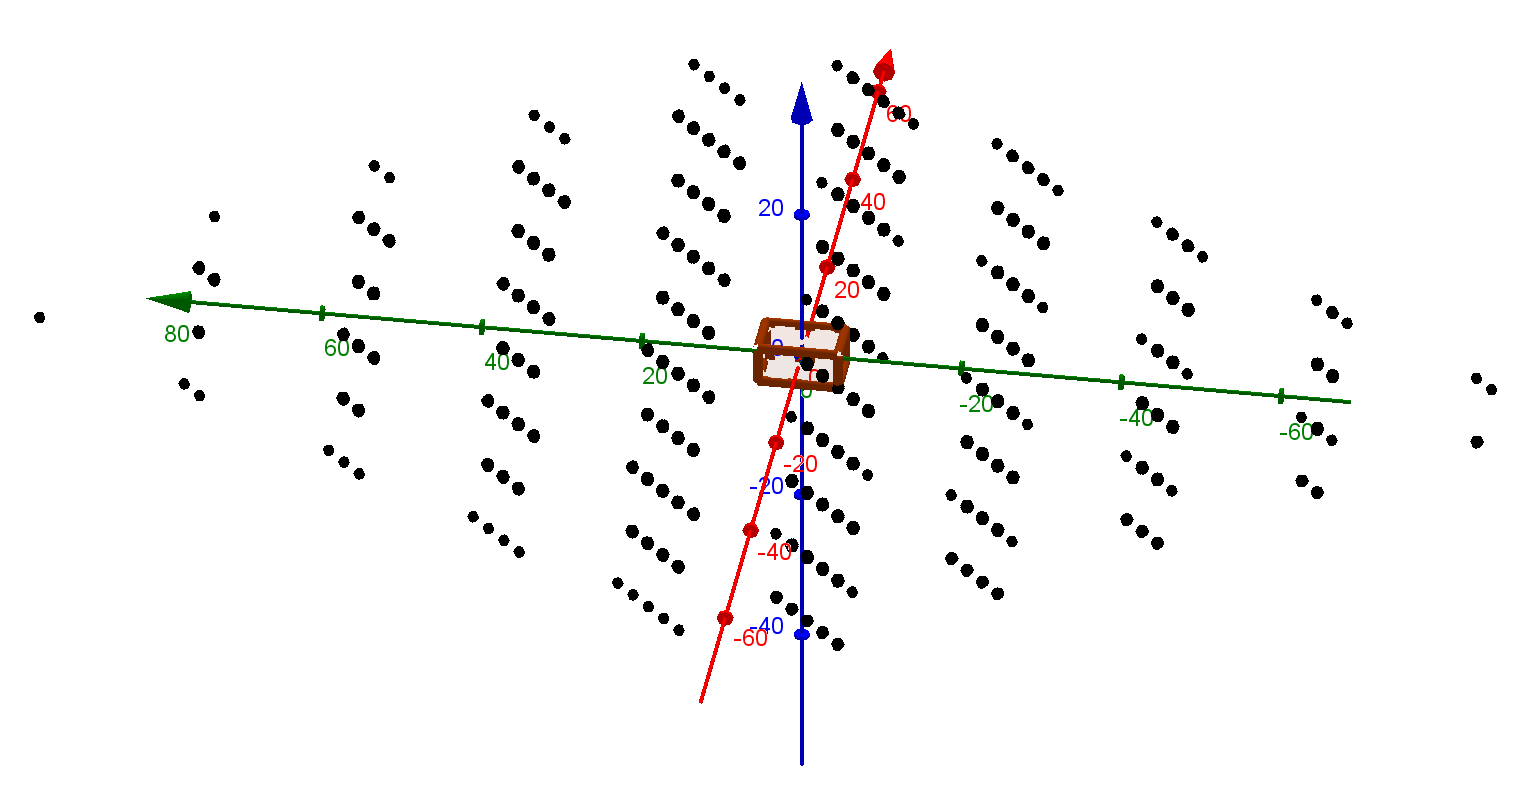
\includegraphics[width=12cm]{siatka2}
	\caption{Siatka źródeł pozornych modelu 2.}
\end{figure}

\begin{figure}[H]
        \centering
                \centering
                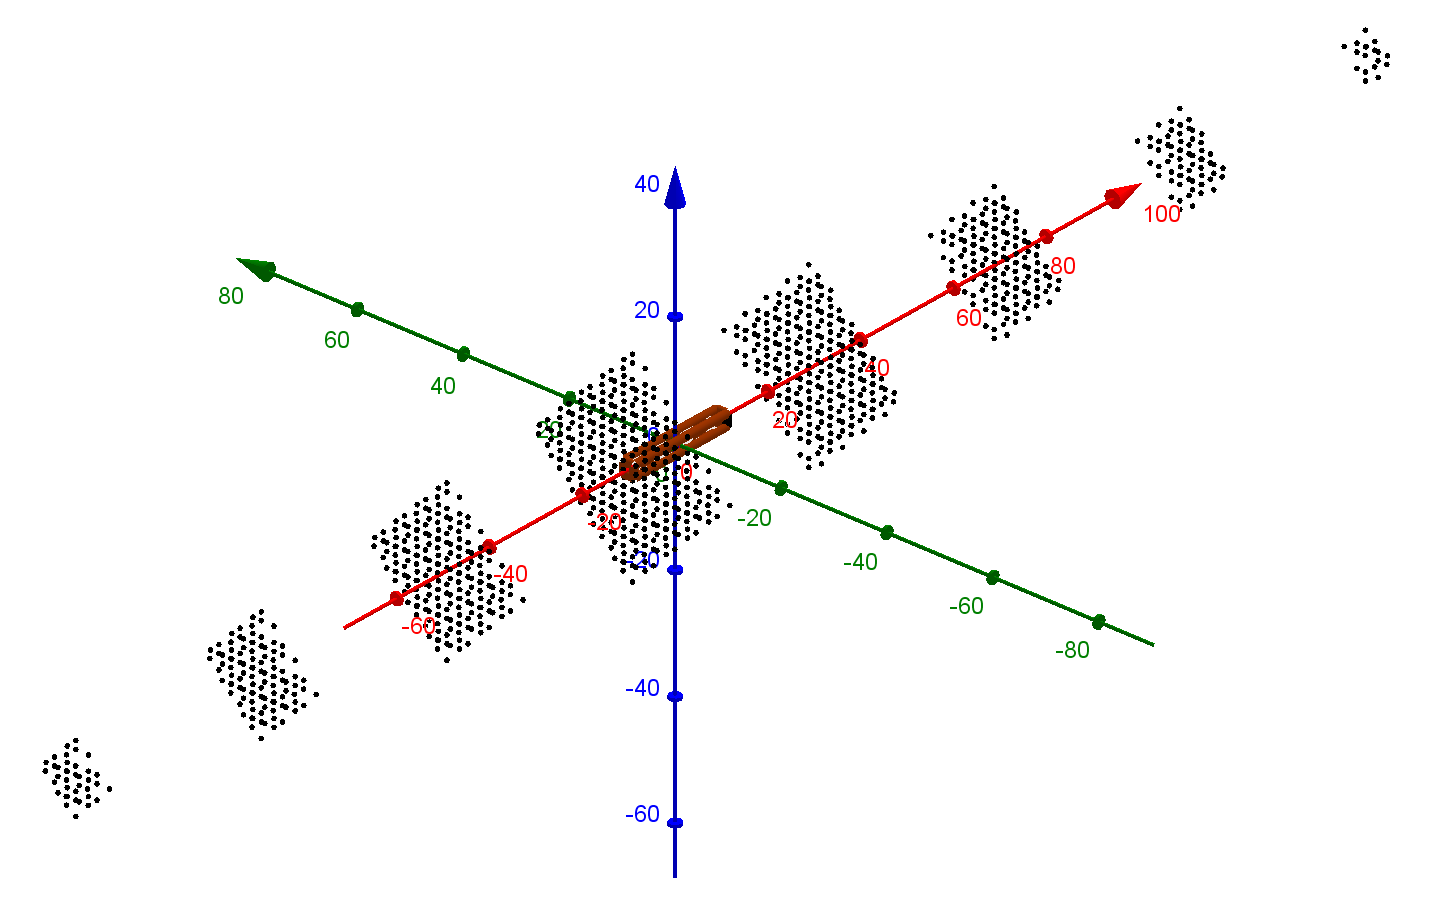
\includegraphics[width=12cm]{siatka3}
	\caption{Siatka źródeł pozornych modelu 3.}
\end{figure}

Na podstawie siatek źródeł pozornych zostały wyznaczone echogramy oraz krzywe zaniku dźwięku (Rys. 6.4-6.9).

\begin{figure}[H]
        \centering
                \centering
                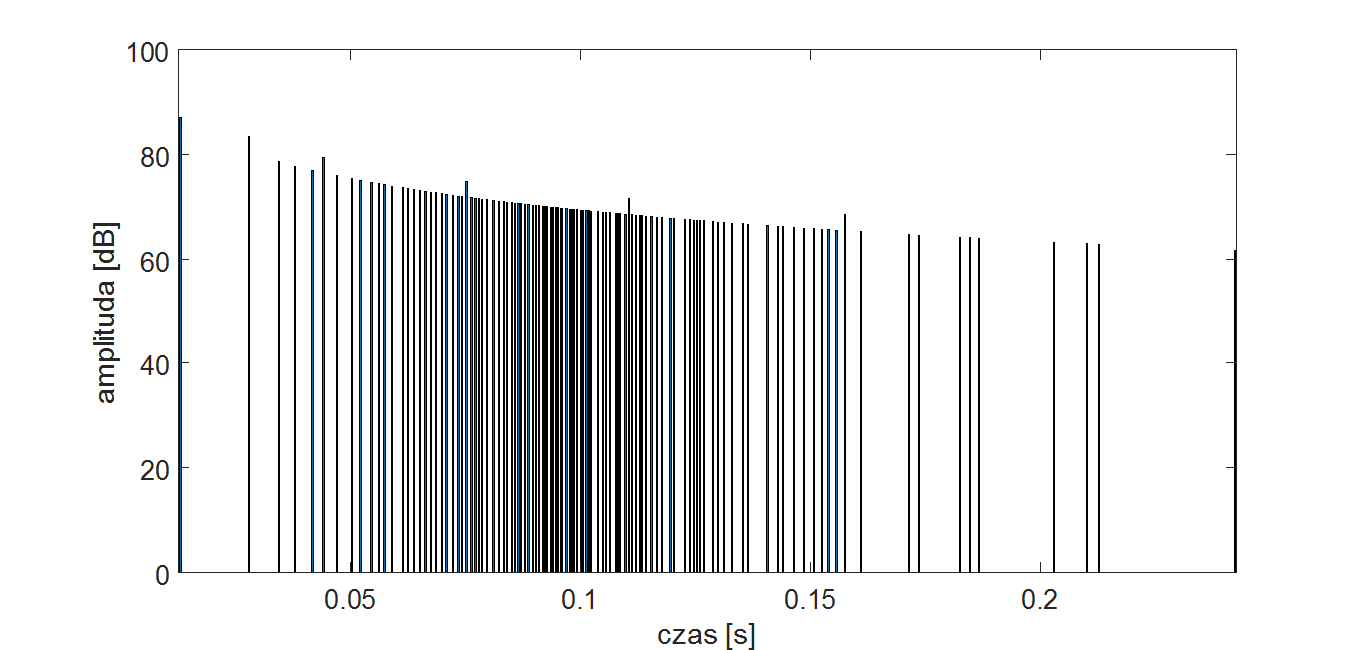
\includegraphics[width=16cm]{echo1}
	\caption{Echogram modelu 1.}
\end{figure}

\begin{figure}[H]
        \centering
                \centering
                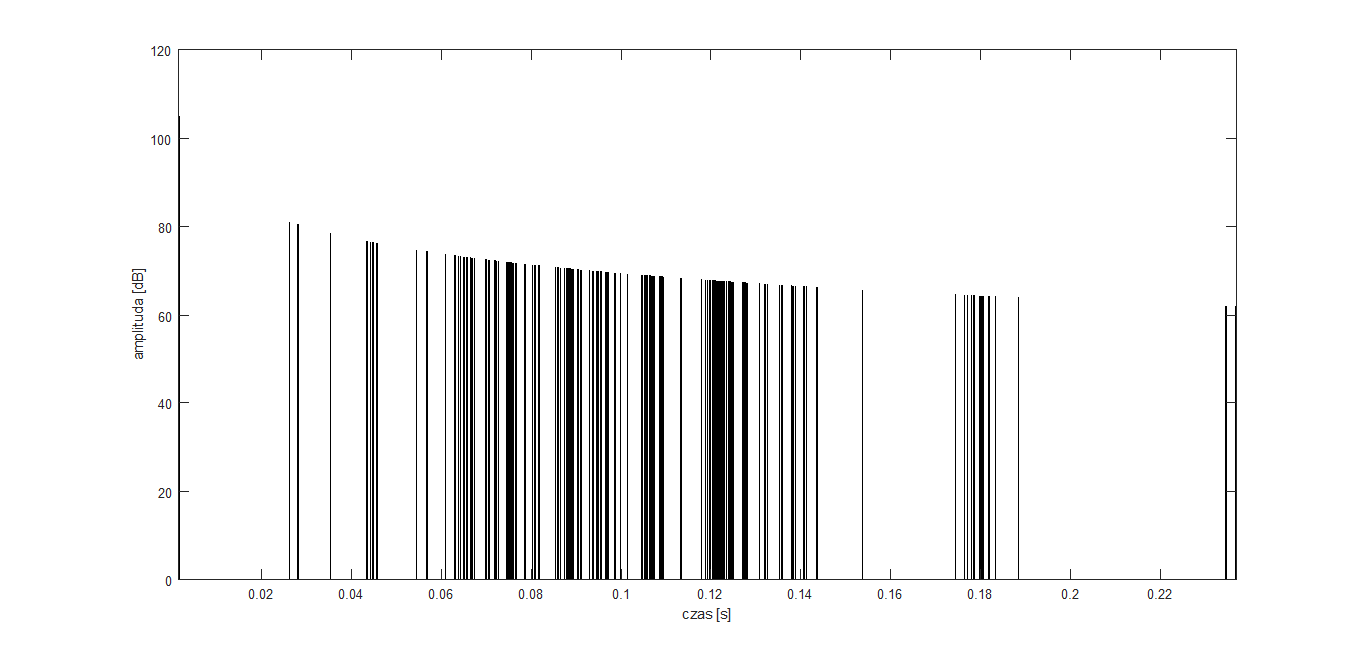
\includegraphics[width=16cm]{echo2}
	\caption{Echogram modelu 2.}
\end{figure}

\begin{figure}[H]
        \centering
                \centering
                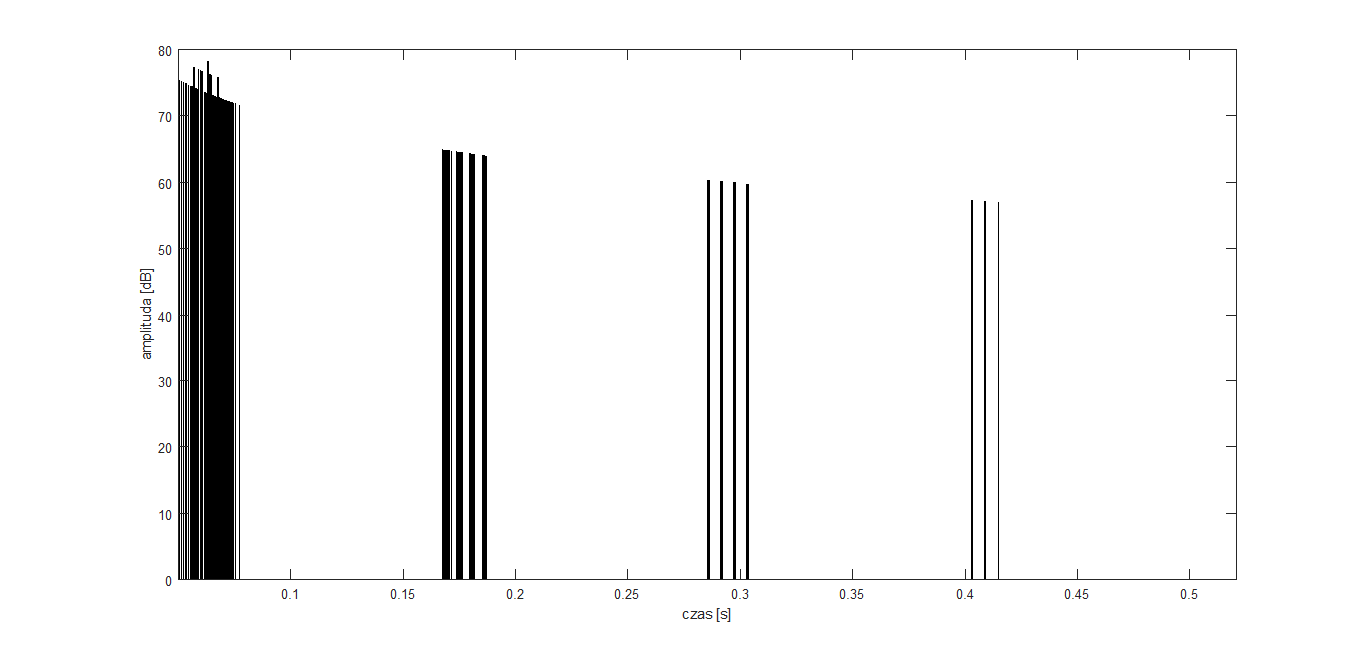
\includegraphics[width=16cm]{echo3}
	\caption{Echogram modelu 3.}
\end{figure}

\begin{figure}[H]
        \centering
                \centering
                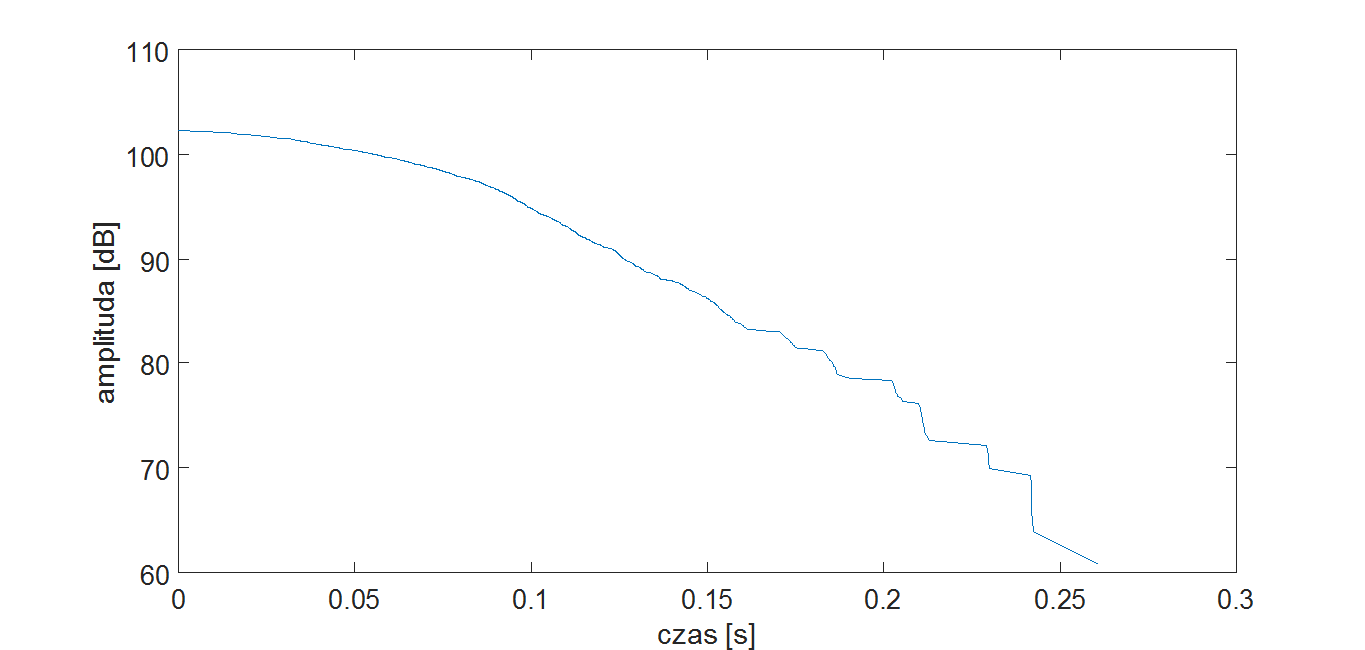
\includegraphics[width=16cm]{zanik1}
	\caption{Krzywa zaniku dźwięku modelu 1.}
\end{figure}

\begin{figure}[H]
        \centering
                \centering
                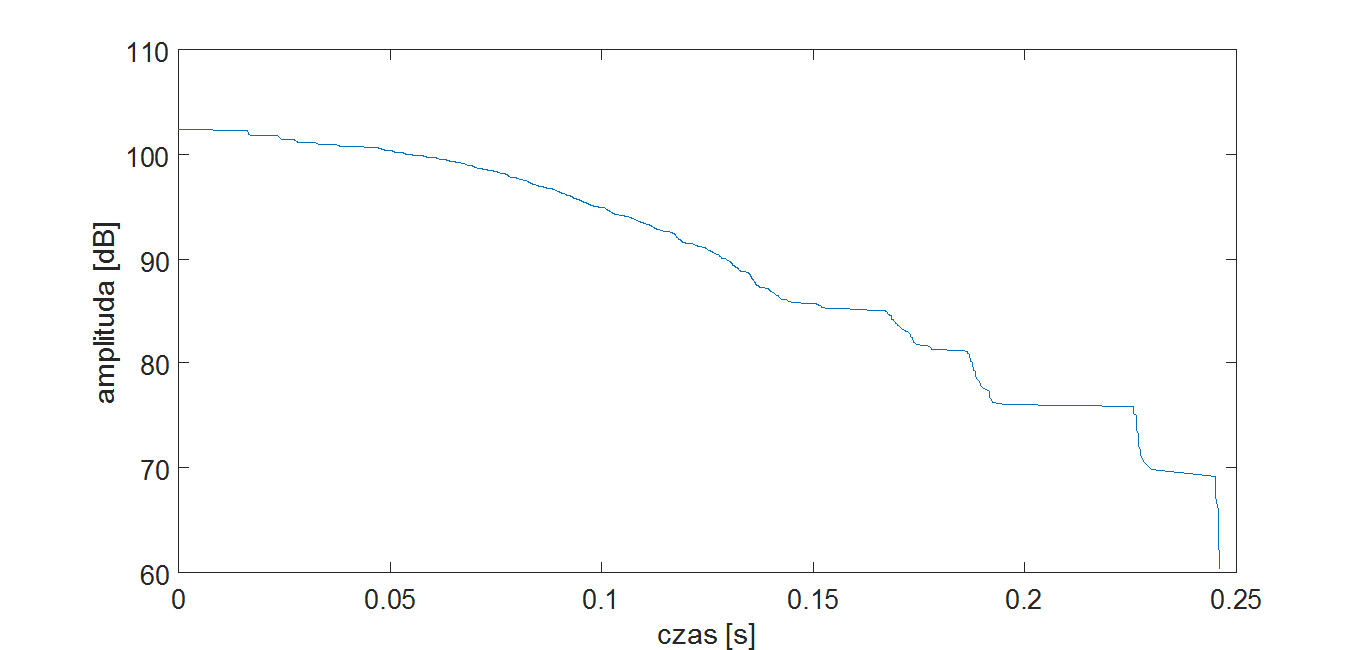
\includegraphics[width=16cm]{zanik2}
	\caption{Krzywa zaniku dźwięku modelu 2.}
\end{figure}

\begin{figure}[H]
        \centering
                \centering
                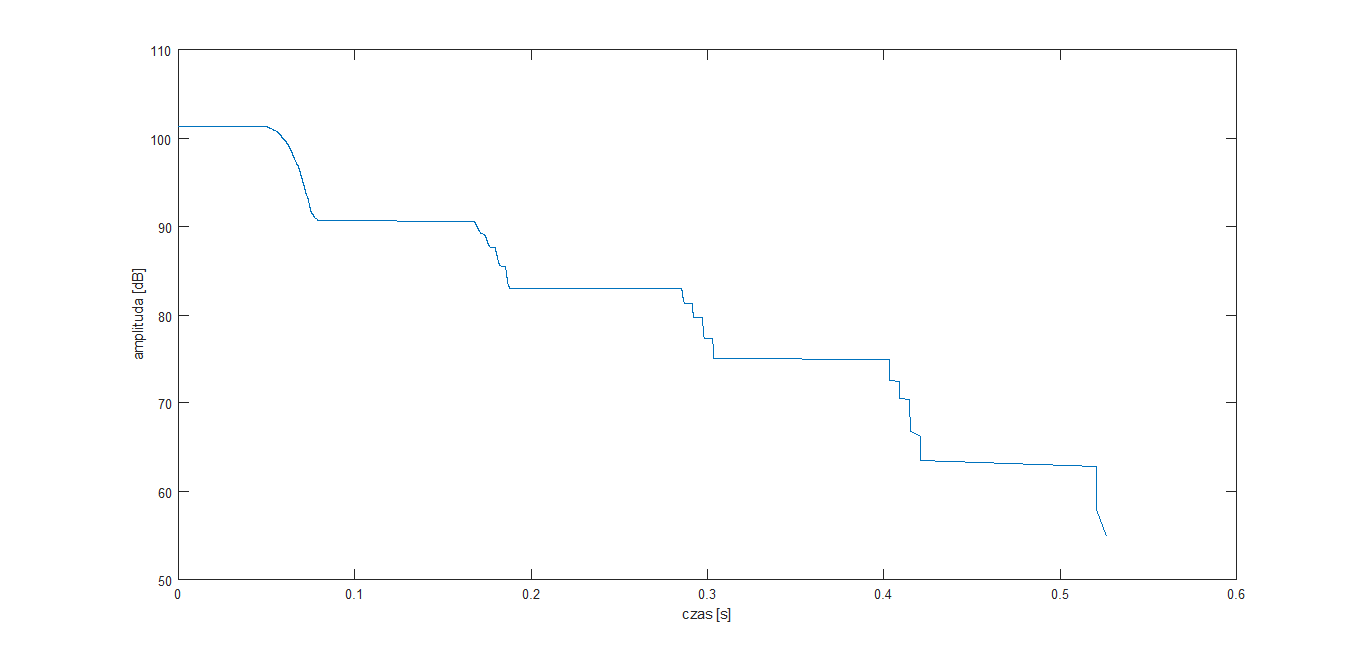
\includegraphics[width=16cm]{zanik3}
	\caption{Krzywa zaniku dźwięku modelu 3.}
\end{figure}


%---------------------------------------------------------------------------

\subsection{Obliczenia na pomieszczeniach o różnych parametrach pochłaniania}\label{sec:imstest2}

Do obliczeń dla zróżnicowanych współczynników pochłaniania wykorzystano model geometryczny 1 z rozdziału 6.2.1. Dla danego modelu zdefiniowano 3 różne zestawy współczynników pochłaniania (Tabela 6.4).

\begin{table}[H]
        \centering
        \begin{threeparttable}
                \caption{Wartośći współczynników pochłaniania dźwięku dla poszczególnych powierzchni w~różnych zestawach danych}\label{tab:table_example}
                \begin{tabularx}{0.6\textwidth}{| c | X | X | X |}
                        \toprule
                        	powierzchnia &	zestaw 1 & zestaw 2 & zestaw 3 \\
                       \midrule
		góra & 0.71 & 0.21 & 0.71 \\
                        dół & 0.78 & 0.18 & 0.78 \\
		lewo & 0.85 & 0.25 & 0.02 \\
                     prawo & 0.72 & 0.12 & 0.72 \\
		przód & 0.84 & 0.24 & 0.84 \\
                    tył & 0.61 & 0.21 & 0.01 \\
                        \bottomrule
                \end{tabularx}
        \end{threeparttable}
\end{table}

Dla danych zestawów siatki źródeł pozornych stanowią te same punkty. Zróżnicowane będą jedynie poziomy poszczególnych promieni dźwiękowych dochodzących do punktu obserwacji, co można zauważyć na echogramach (Rys. 6.10-6.12).

\begin{figure}[H]
        \centering
                \centering
                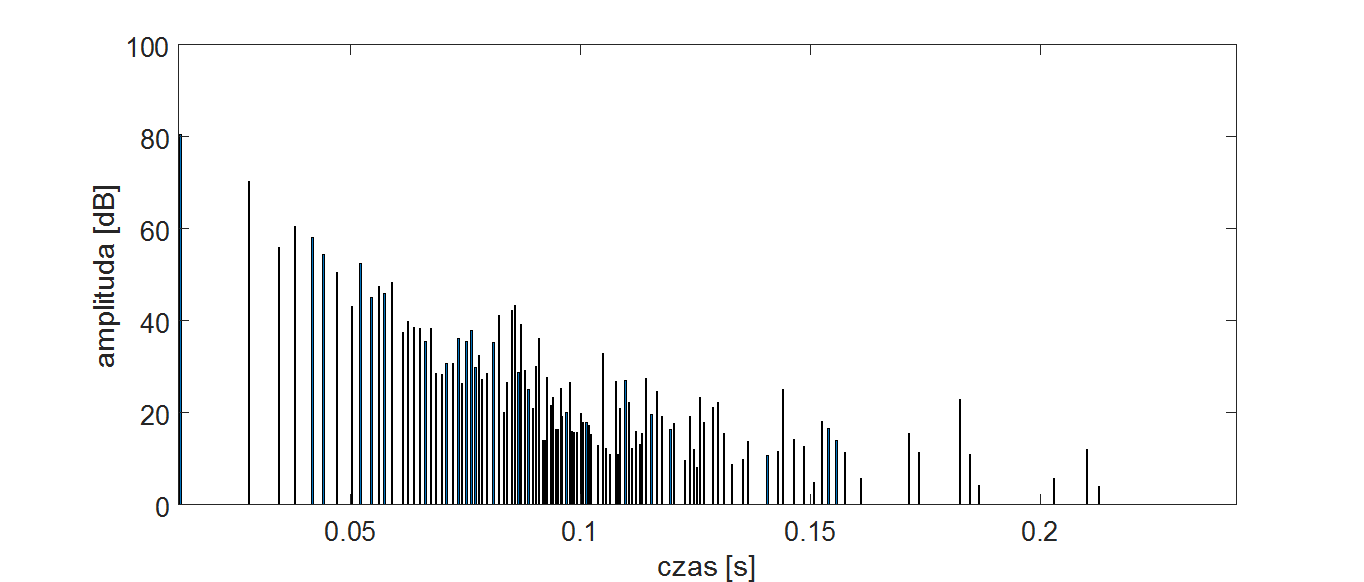
\includegraphics[width=16cm]{echoz1}
	\caption{Echogram modelu 1.}
\end{figure}

\begin{figure}[H]
        \centering
                \centering
                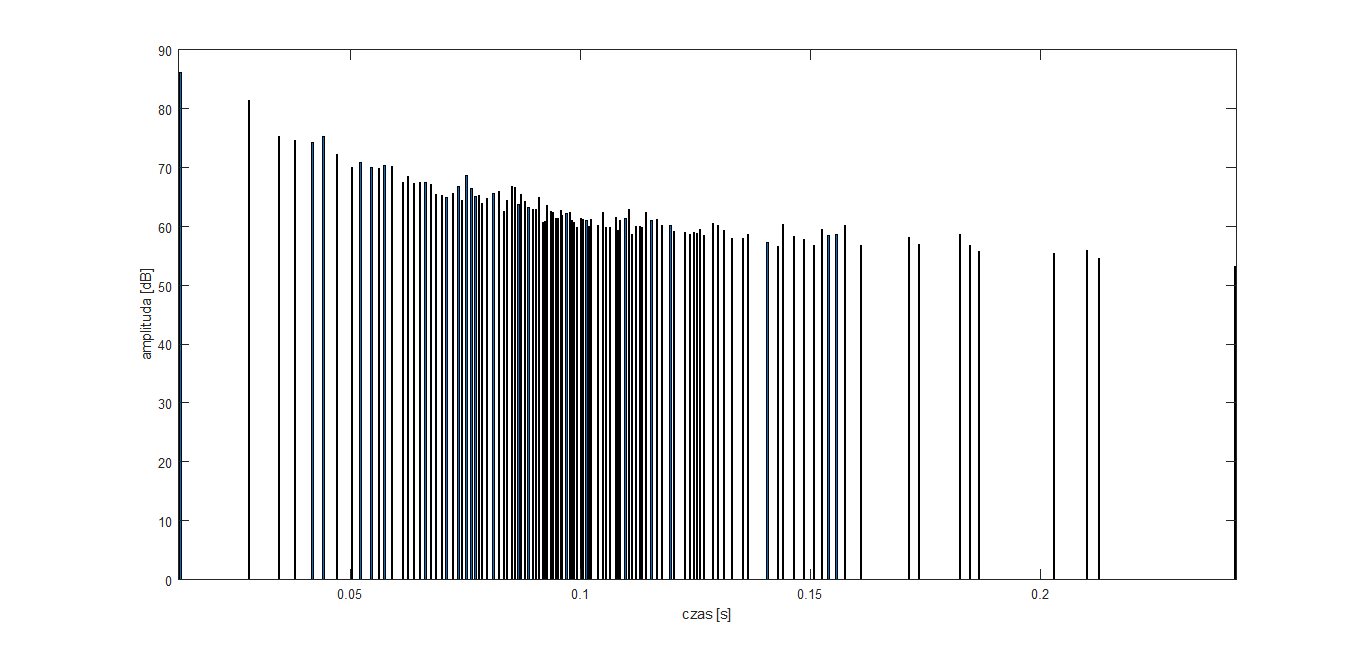
\includegraphics[width=16cm]{echo2z}
	\caption{Echogram modelu 2.}
\end{figure}

\begin{figure}[H]
        \centering
                \centering
                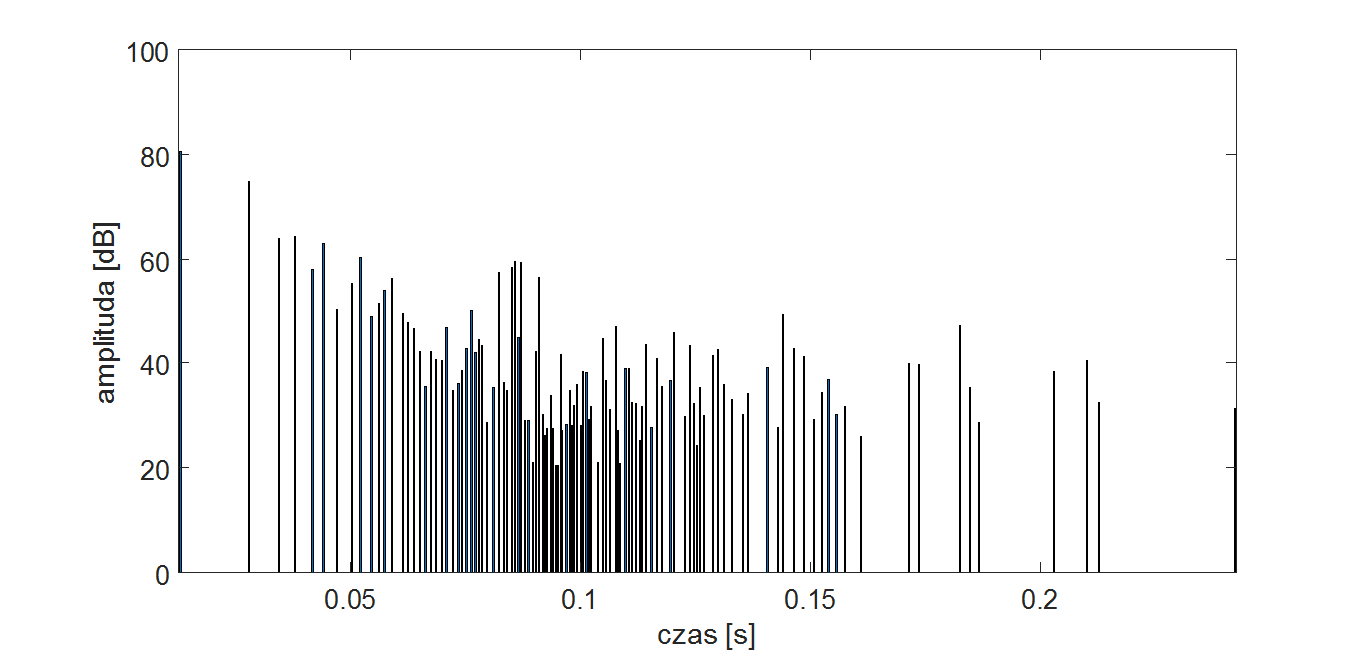
\includegraphics[width=16cm]{echoz3}
	\caption{Echogram modelu 3.}
\end{figure}

Różne parametry pochłaniania mają wpływ na kształt i~szybkość zanikania krzywej zaniku dźwięku (Rys. 6.13-6.15).

\begin{figure}[H]
        \centering
                \centering
                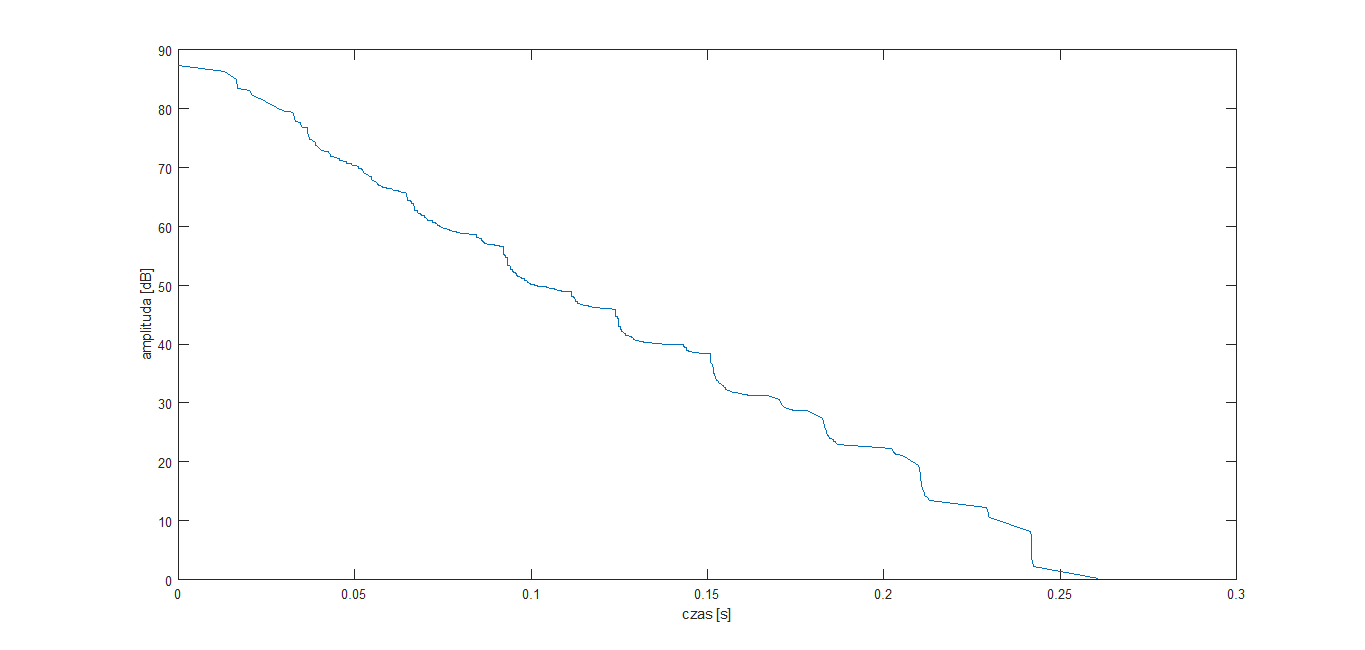
\includegraphics[width=16cm]{zanikz1}
	\caption{Krzywa zaniku dźwięku modelu 1.}
\end{figure}

\begin{figure}[H]
        \centering
                \centering
                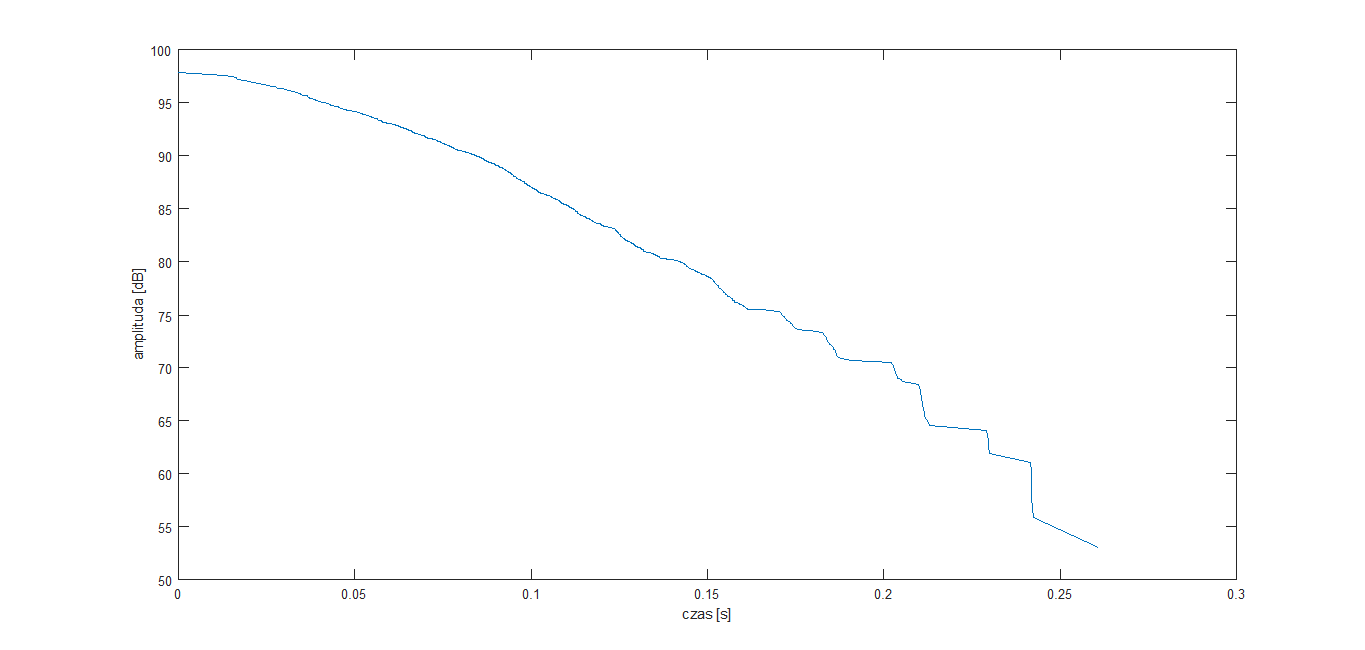
\includegraphics[width=16cm]{zanikz2}
	\caption{Krzywa zaniku dźwięku modelu 2.}
\end{figure}

\begin{figure}[H]
        \centering
                \centering
                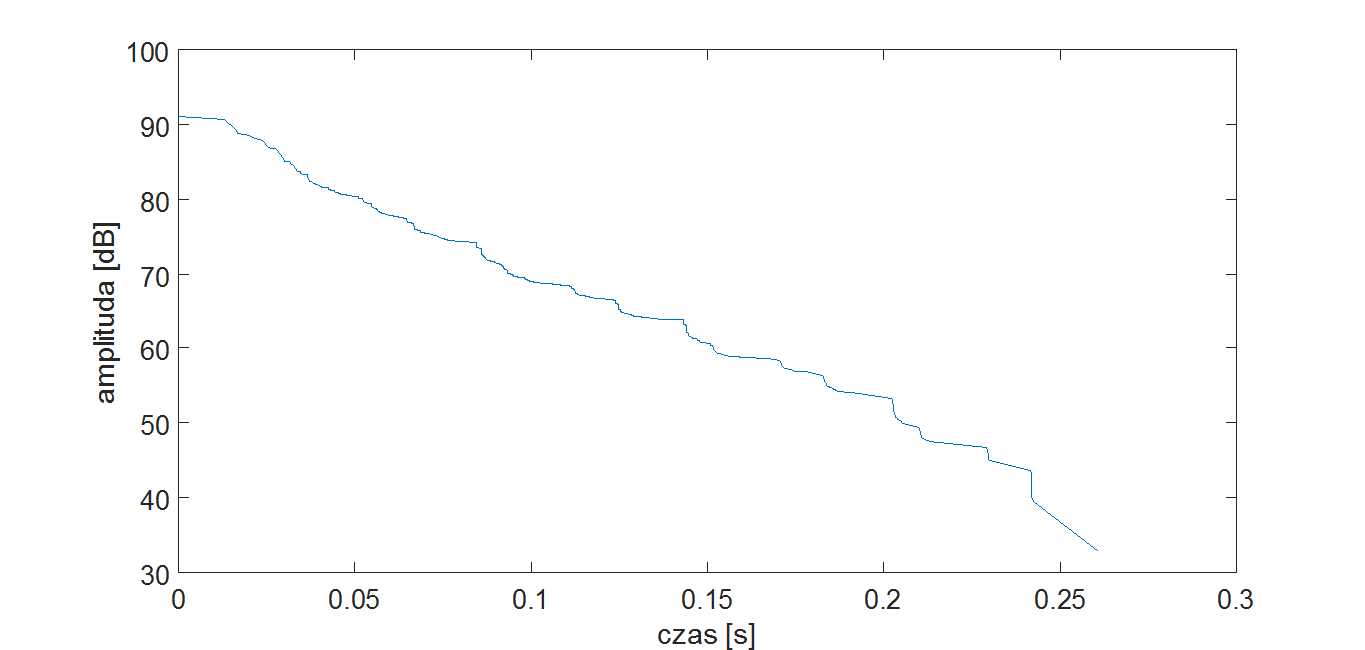
\includegraphics[width=16cm]{zanikz3}
	\caption{Krzywa zaniku dźwięku modelu 3.}
\end{figure}

%---------------------------------------------------------------------------

\subsection{Wizualizacja poszczególnych promieni dźwiękowych}\label{sec:imstest2}

Podczas testów aplikacji użyteczna okazała się możliwość wizualizacji ścieżki wybranego promienia dźwiękowego. Aplikacja autora pracy umożliwia wygenerowanie skryptu jako plik wejściowy do programu GeoGebra, który umożliwia prezentację ścieżki promienia dźwiękowego dla wybranych wariacji powierzchni odbijających (Rysunek 6.16 - 6.19.).  

\begin{figure}[H]
        \centering
                \centering
                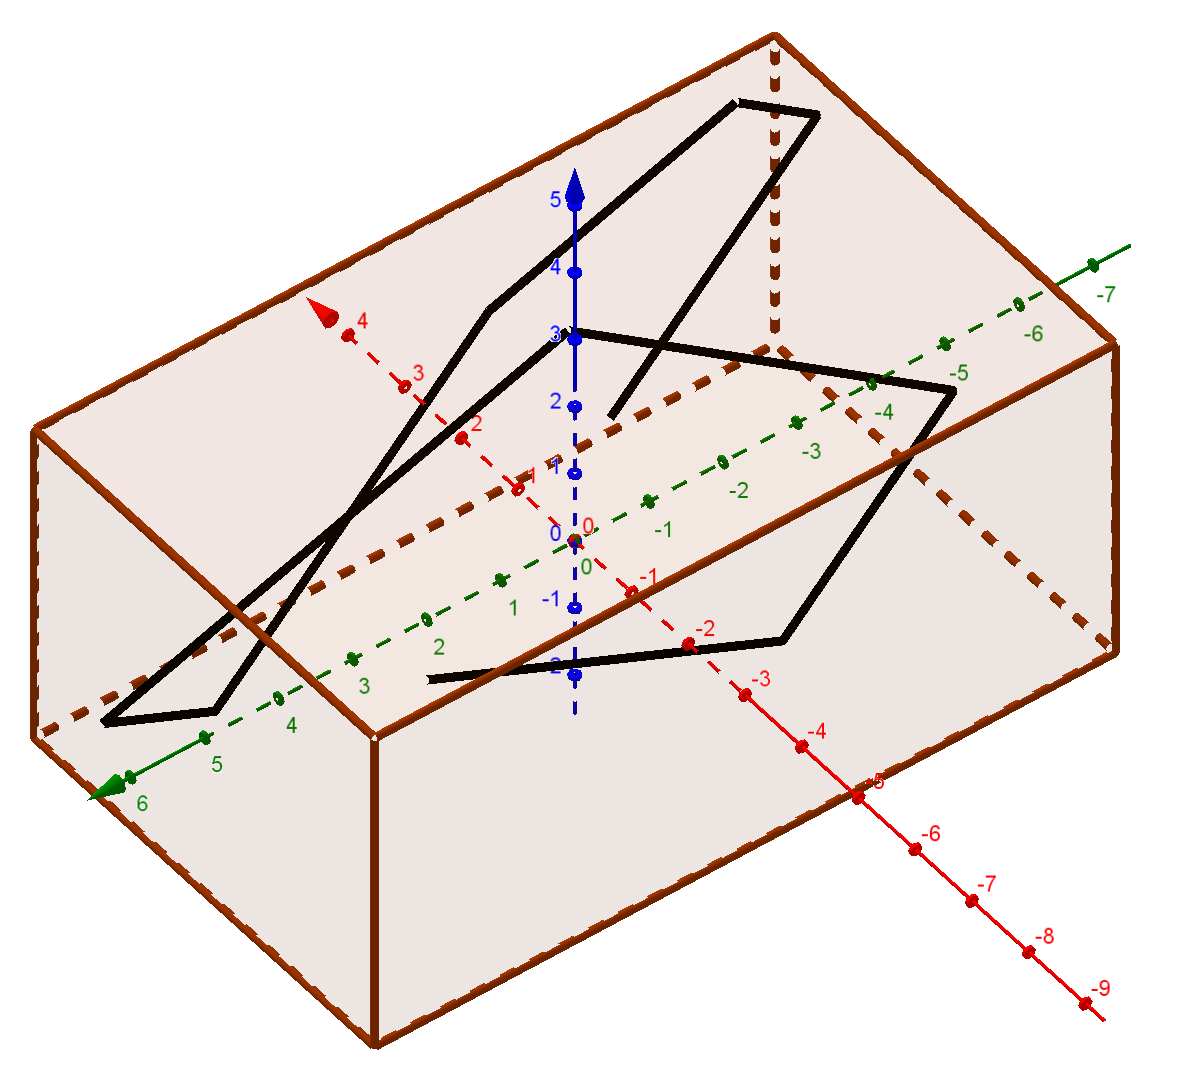
\includegraphics[width=12cm]{odbicia}
	\caption{Ścieżka wybranego promienia dźwiękowego dla 8 odbić.}
\end{figure}

\begin{figure}[H]
        \centering
                \centering
                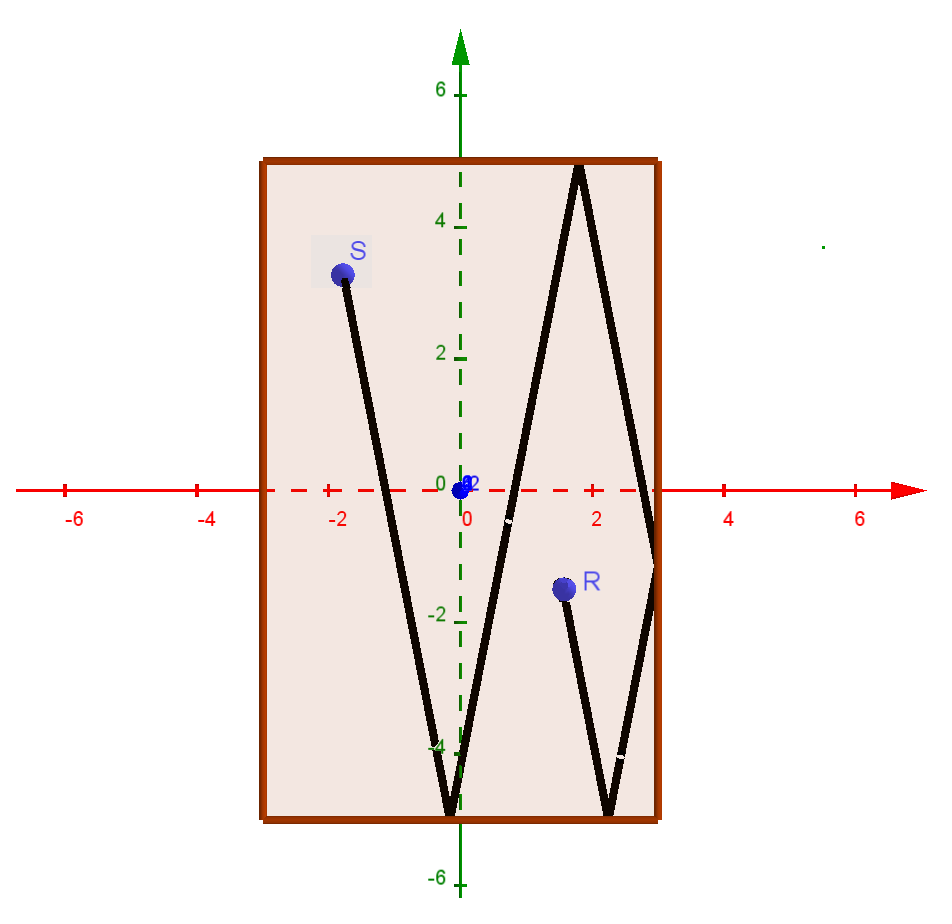
\includegraphics[width=12cm]{odbiciaz}
	\caption{Ścieżka wybranego promienia dźwiękowego dla 8 odbić w~rzucie na płaszczyznę XY (S - punkt źródła dźwięku, R - punkt obserwacji).}
\end{figure}

\begin{figure}[H]
        \centering
                \centering
                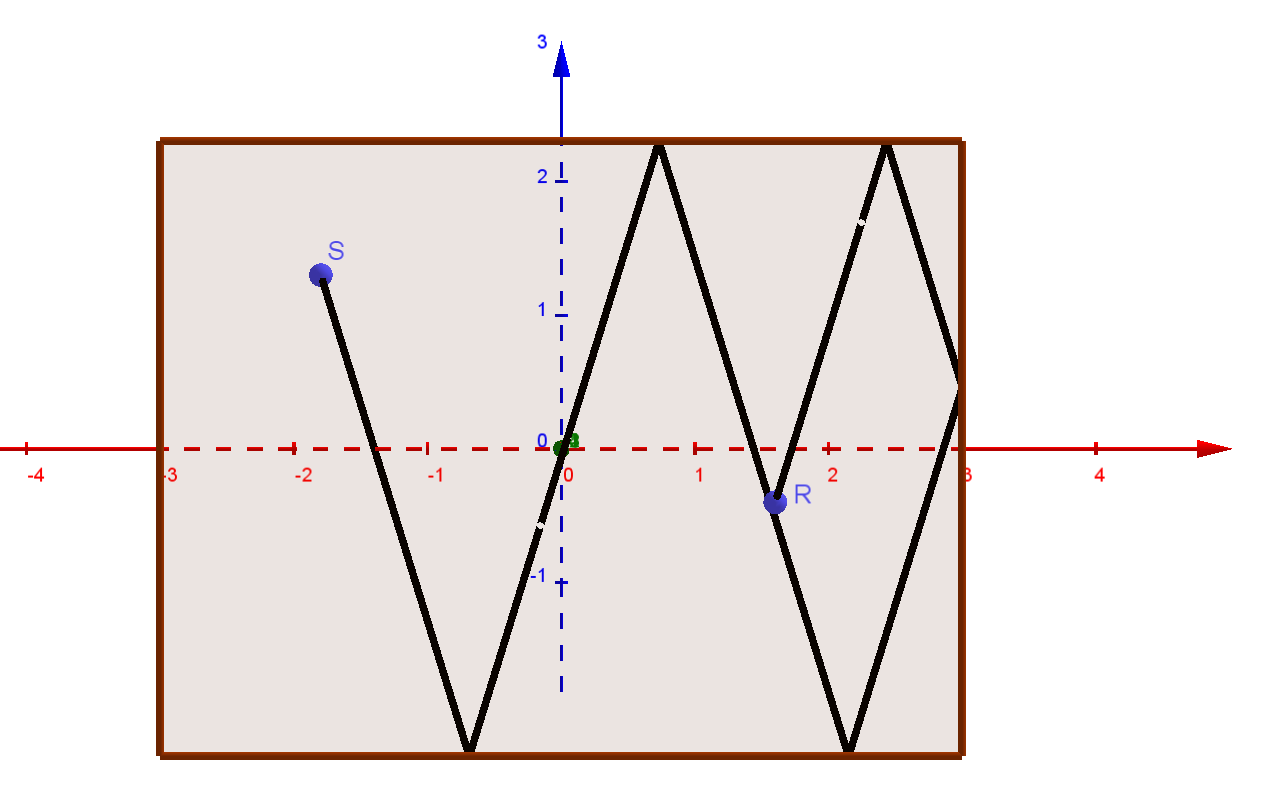
\includegraphics[width=12cm]{odbiciay}
	\caption{Ścieżka wybranego promienia dźwiękowego dla 8 odbić w~rzucie na płaszczyznę XZ (S - punkt źródła dźwięku, R - punkt obserwacji).}
\end{figure}

\begin{figure}[H]
        \centering
                \centering
                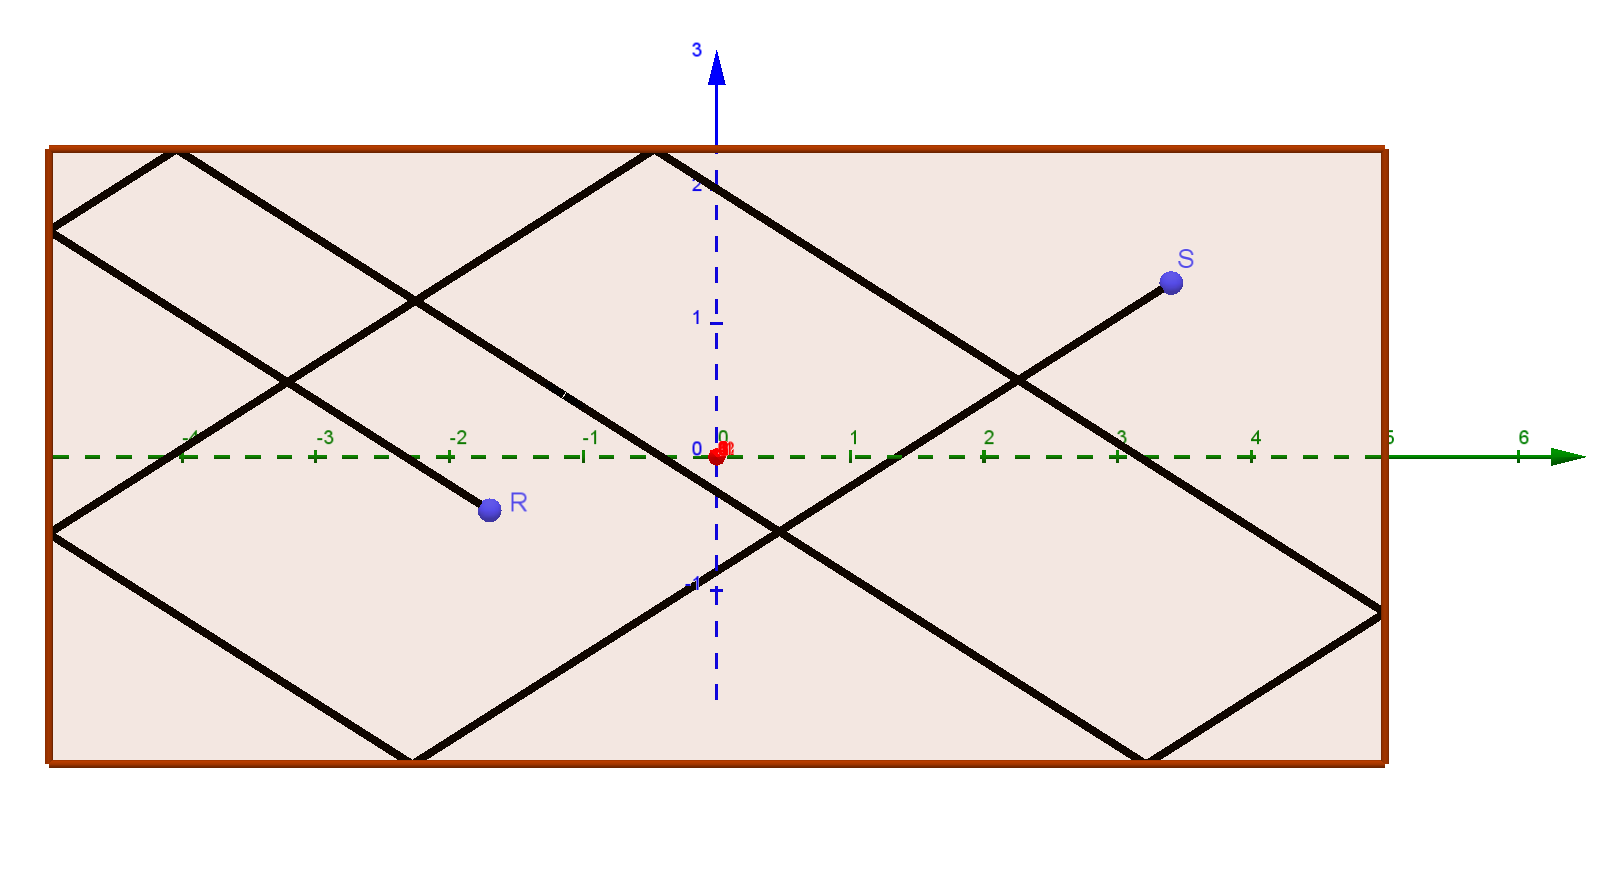
\includegraphics[width=12cm]{odbiciax}
	\caption{Ścieżka wybranego promienia dźwiękowego dla 8 odbić w~rzucie na płaszczyznę YZ (S - punkt źródła dźwięku, R - punkt obserwacji).}
\end{figure}

Wizualizacja ścieżek promieni dźwiękowych może być przydatna w~akustyce architektonicznej przy projektowaniu rozmieszczenia ustrojów akustycznych. Rysując promienie dźwiękowe dla pierwszych odbić (Rysunek 6.20.) możemy wyznaczyć punkty, w~których dane odbicia zachodzą. Umieszczając materiał o innych właściwościach pochłaniania w~miejscach pierwszych odbić możemy wpłynąć na ilość energii jaka przychodzi do odbiornika w~pierwszych milisekundach, co pozwala bezpośrednio wpłynąć na wskaźniki C50, C80, D50 oraz wskaźnik zrozumiałości mowy.

\begin{figure}[H]
        \centering
                \centering
                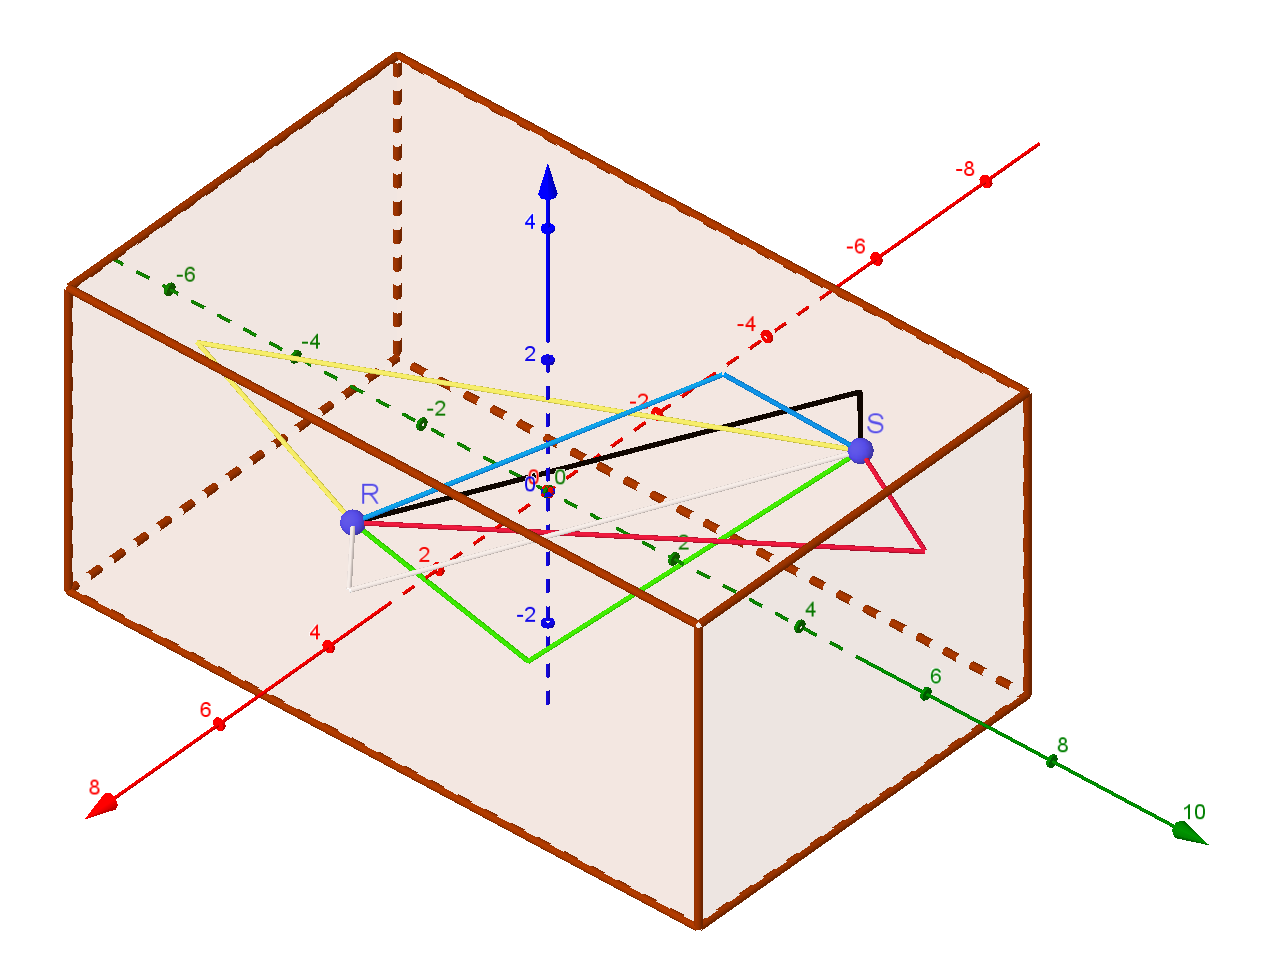
\includegraphics[width=12cm]{1szeodbicia}
	\caption{Ścieżki promieni dźwiękowych dla pierwszych odbić (S - punkt źródła dźwięku, R - punkt obserwacji).}
\end{figure}

\begin{figure}[H]
        \centering
                \centering
                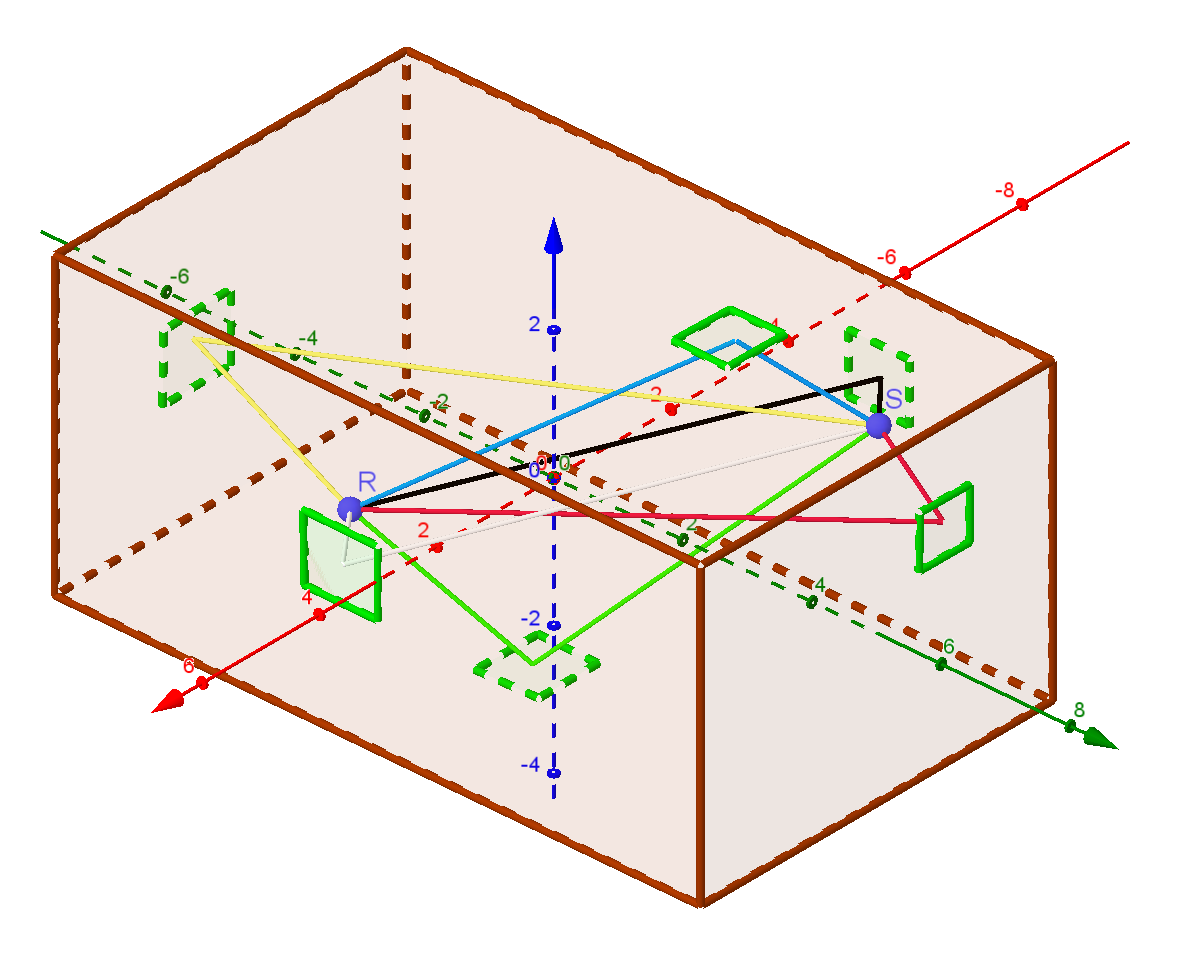
\includegraphics[width=12cm]{1odbiciazpoch}
	\caption{Ścieżki promieni dźwiękowych dla pierwszych odbić wraz z rozmieszczeniem materiałów pochłaniających (S - punkt źródła dźwięku, R - punkt obserwacji).}
\end{figure}

Dla tak przygotowanych modeli możemy wyznaczyć echogramy (Rysunek 6.21 - 6.22.) i~ilość energii, która dochodzi do punktu obserwacji. Pozwala to na dostrojenie modelu do wybranych założeń projektowych, jakimi mogą być wartości wcześniej wymienionych wskaźników.

\begin{figure}[H]
        \centering
                \centering
                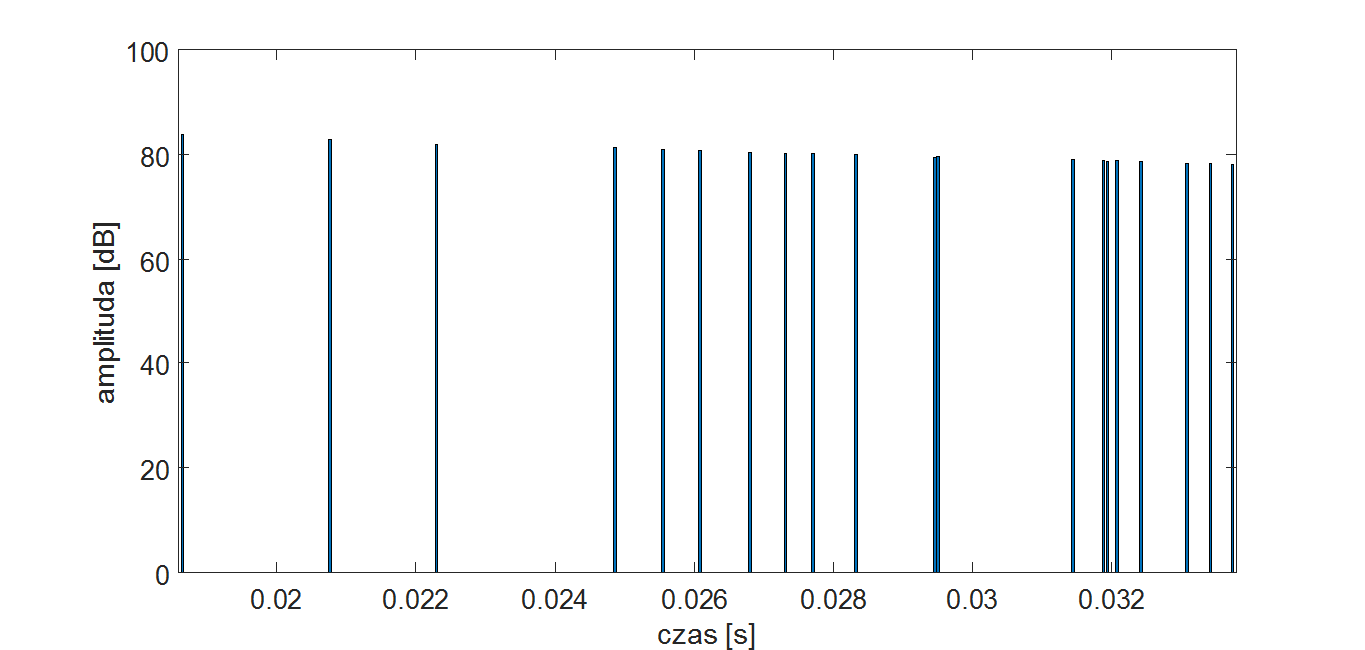
\includegraphics[width=16cm]{echogramodbicia}
	\caption{Echogram dla 20 pierwszych odbić.}
\end{figure}

\begin{figure}[H]
        \centering
                \centering
                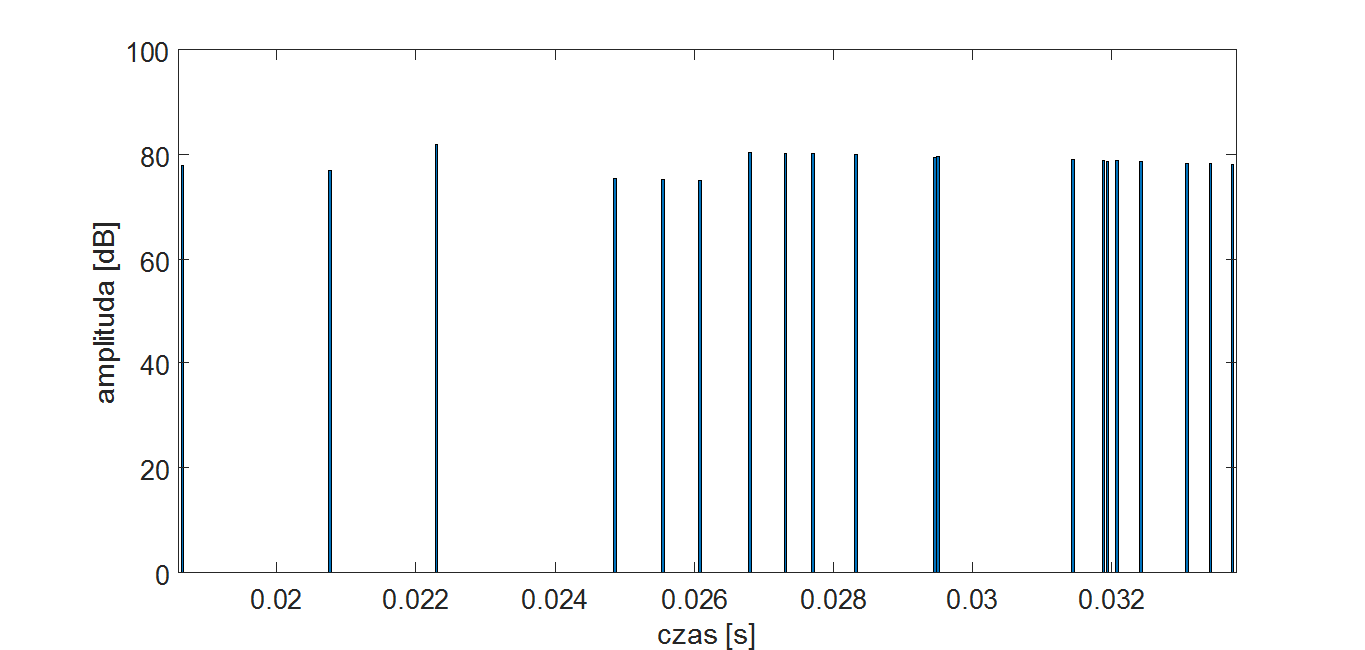
\includegraphics[width=16cm]{echogramodbiciazpoch}
	\caption{Echogram dla 20 pierwszych odbić dla modelu z ustrojami pochłaniającymi.}
\end{figure}

%---------------------------------------------------------------------------

\section{Testy wydajnościowe}\label{sec:asdas2d}

Testy wydajnościowe przeprowadzono na 2 różnych architekturach procesorów – CPU i~GPU. Do pomiarów na CPU posłużył procesor Intel Core i5-2520M (Tabela 6.5). Pomiaru przy użyciu GPU przeprowadzono na kartach Radeon R7 250X (Tabela 6.6) oraz Radeon R9 270X (Tabela 6.7). Obliczenia testowe zostały wykonane na zmiennych o pojedynczej precyzji.
 
\begin{table}[H]
        \centering
        \begin{threeparttable}
                \caption{Dane techniczne procesora Intel Core i5-2520M}\label{tab:table_example}
                \begin{tabularx}{0.6\textwidth}{| c | X |}
                       \midrule
		taktowanie & 2,50 GHz \\
                     liczba rdzeni & 2 \\
                    liczba wątków & 4 \\
                        \bottomrule
                \end{tabularx}
        \end{threeparttable}
\end{table}

\begin{table}[H]
        \centering
        \begin{threeparttable}
                \caption{Dane techniczne karty graficznej Radeon R7 250x}\label{tab:table_example}
                \begin{tabularx}{0.6\textwidth}{| c | X |}
                       \midrule
		taktowanie & 1000 MHz \\
                     liczba rdzeni GPU & 512 \\
                        \bottomrule
                \end{tabularx}
        \end{threeparttable}
\end{table}

\begin{table}[H]
        \centering
        \begin{threeparttable}
                \caption{Dane techniczne karty graficznej Radeon R9 270x}\label{tab:table_example}
                \begin{tabularx}{0.6\textwidth}{| c | X |}
                       \midrule
		taktowanie & 1030 MHz \\
                     liczba rdzeni GPU & 2560 \\
                        \bottomrule
                \end{tabularx}
        \end{threeparttable}
\end{table}

Pomiary przeprowadzono na modelu 1 z rozdziału 6.2.1 (Rysunek~6.1.) dla rzędów źródeł pozornych od 5 do 12. Autor porównał ze sobą czasy obliczeń na różnych platformach (Rysunek~6.13.,~Tabela~6.8.).

\begin{figure}[H]
        \centering
                \centering
                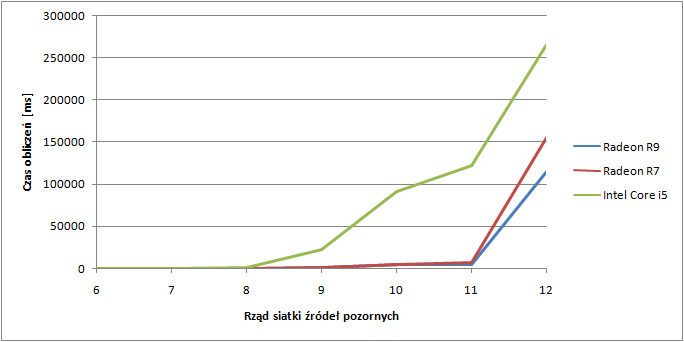
\includegraphics[width=16cm]{wykres}
	\caption{Zależność czasu obliczeń od liczby wyliczanych rzędów siatki źródeł pozornych dla różnych urządzeń.}
\end{figure}

W celu sprawdzenia wydajności implementacji algorytmu w~środowisku OpenCL autor porównał czas obliczeń algorytmu w~tym środowisku z czasem obliczeń algorytmu zaimplementowanego przy użyciu czystego kodu C++, bez użycia wielowątkowości (Rysunek~6.14.,~Tabela~6.9.).

\begin{figure}[H]
        \centering
                \centering
                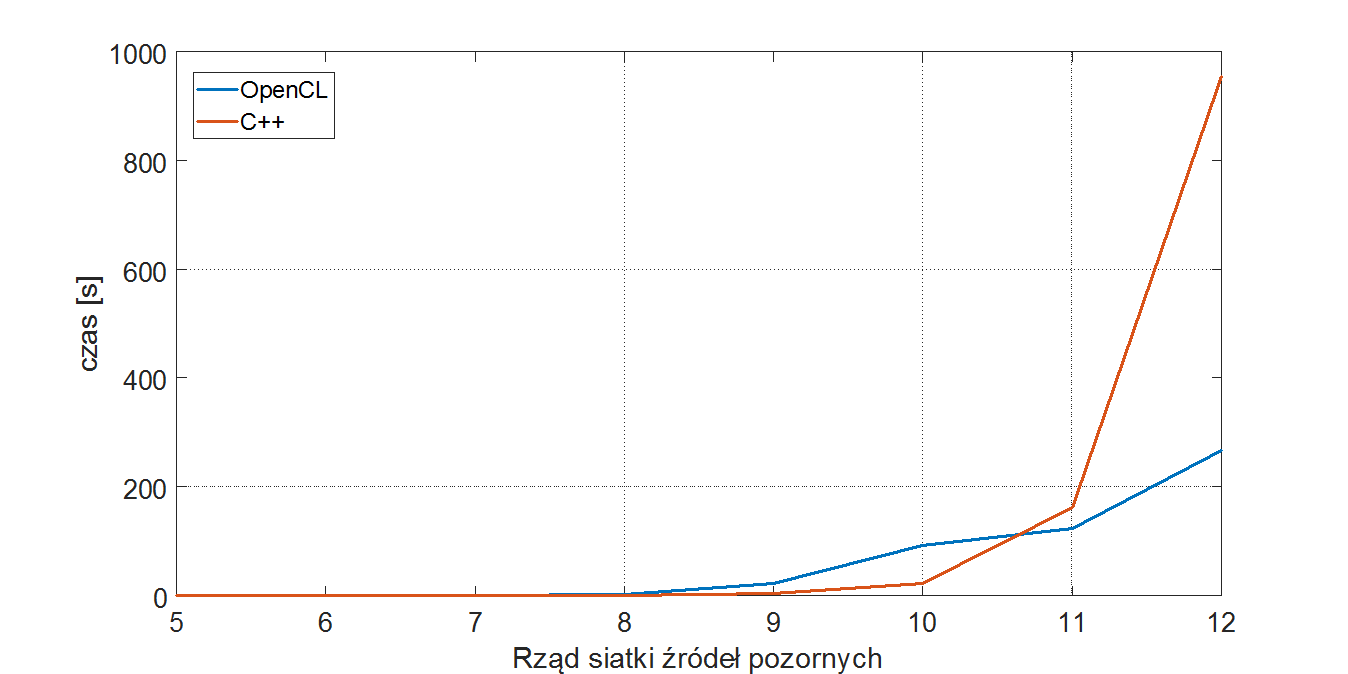
\includegraphics[width=16cm]{wykres2}
	\caption{Zależność czasu obliczeń od używanego środowiska na tej samej platformie sprzętowej.}
\end{figure}


%---------------------------------------------------------------------------

\section{Błąd obliczeń}\label{sec:asdas2sd}

Większa część algorytmu metody źródeł pozornych odpowiada za sprawdzenie czy dany promień dźwiękowy istnieje w~danym modelu geometrycznym. Sprawdzenie odpowiada jedynie za decyzję czy dany promień będzie uwzględniany w~siatce źródeł pozornych i~nie wpływa na błąd wyniku końcowego. Błąd obliczonych pozycji siatki źródeł pozornych powstaje w~wyniku narastania błędu zaokrąglenia podczas operacji arytmetycznych związanych z wyznaczaniem kolejnych odbić lustrzanych punktu źródła. Do obliczenia współrzędnej odbicia należy wykonać 4 mnożenia co czterokrotnie zwiększa wartość błędu względnego $\epsilon$. Dla współrzędnych zapisanych w~zmiennych typu float daje to błąd względny równy |$\delta$| = 2 E-21. Dla źródeł pozornych N-tego rzędu wartość tego błędu wzrasta o N razy. Nawet dla źródeł pozornych 16-tego rzędu błąd wynosi |$\delta$| = 2 E-17. W akustyce architektonicznej błędy danych wejściowych są o kilkanaście rzędów wielkości większe od tego błędu przez co może on zostać pominięty w~obliczeniach.\\









\chapter{Podsumowanie}\label{cha:podsum}

W ramach pracy napisana została aplikacja, która implementuje metodę źródeł pozornych na heterogeniczne platformy obliczeniowe. Wyniki testów wydajności z rozdziału 5.3 wykazały, że obliczenia algorytmu zaimplementowanego w~OpenCL wykonane z użyciem kart graficznych są znacznie szybsze niż na zwykłych procesorach i~możliwa jest optymalizacja tej metody wykorzystując bardziej złożone platformy. Algorytm napisany w~OpenCL na procesorze CPU wykonuje się szybciej niż algorytm napisany w~czystym języku C++ dla rzędu odbić powyżej 11. Przy małej ilości odbić na szybkość algorytmu wpływa głównie czas dostępu do pamięci, który jest znacznie krótszy przy jednowątkowych aplikacjach.    

Wykorzystanie popularnej biblioteki OpenCL i~prezentacja aplikacji w~postaci otwartego kodu umożliwia wykorzystanie jej w~innych aplikacjach  lub do niezależnych badań. Otwarty kod kernela pozwala na implementacje programu w~dowolnym języku platformy obsługiwanym przez standard OpenCL (m. in. Python, Matlab).

Obliczenia w~rozdziale 5.2 ukazują użyteczność aplikacji w~analizie pomieszczeń. Analiza wyznaczonych echogramów pozwala na wstępną ocenę warunków akustycznych pomieszczenia i~daje informacje o wczesnych odbiciach. Użycie zewnętrznej nakładki graficznej w~programie GeoGebra pozwoliło na analizę poszczególnych odbić, co może być użyteczne przy projektowaniu rozmieszczenia ustrojów akustycznych w~pomieszczeniu. Wyznaczone siatki źródeł pozornych mogą posłużyć do dalszej analizy warunków akustycznych i~wyznaczenia wskaźników C50, C80, D50, wskaźnika zrozumiałości mowy i~innych parametrów nie rozpatrzonych w~pracy.
%\chapter{Testy}

\section{Test URL-a}

Wejdź na stronę \url{https://www.google.pl/} i wpisz szukane zdanie.

\clearpage

\section{Test dzielenia wdów}

Lorem ipsum dolor sit amet, ex est alia dolorem commune. Duo modo errem no. Ea harum doming atomorum mei. Consul animal malorum cu qui, sumo dicta graece an est, vim ei clita regione.

Vel eu quando doming fastidii, mei graeco indoctum an, legere theophrastus in pro. Te mei probatus eleifend interpretaris. Est no autem liber vituperatoribus, cu mea dicam constituto. Ea laudem tritani consectetuer sit, sanctus patrioque expetendis vix in. Duo id fugit adversarium signiferumque, an quot modus molestiae qui.

Ut paulo definiebas pro. Mea an quod esse. Et atomorum facilisis moderatius sit. Graeco iudicabit forensibus in vel. Eam cu lorem aeterno offendit, cu vix nulla congue posidonium. Vel lucilius evertitur vituperata no.

Mea eu graecis prodesset. Et tota eius nec. Ei etiam oratio has, vel ei homero eripuit invenire. Sed ex errem intellegebat, sea et elitr intellegat constituto. Nostro voluptua accusamus eos in, ei sale admodum has. Vim ne consetetur reformidans, ad has malis recusabo persequeris, per etiam virtute invenire in.

Te nihil eruditi eam, sit aperiam accusam mediocritatem at. Nec ne nonumy dictas disputationi, vis ridens sadipscing ex. Harum euripidis ex vix, at consetetur instructior signiferumque mel, at mei elitr honestatis. Id sit congue vituperata. Temporibus eloquentiam no eum.

Pro id esse phaedrum, nostro iudicabit eos ut. Sit ea aperiam alienum, harum audiam voluptua cu usu. Iudico invenire te vel, id suscipit disputando pri. Ut sumo expetenda mea.

Cum at idque nullam aperiam, vis ex aeque ponderum luptatum. Vix soluta graeco dissentiet ut, ut est reque periculis similique, ut dicta dicant repudiare sea. Ne dolor legendos signiferumque ius, at eirmod convenire qui. Suas numquam conceptam mei ex. Autem homero eos et, sea dicta alienum iudicabit ut.

Ea duo consulatu vulputate, id elit perpetua cum. His ei aeque saepe audiam. Prompta laoreet facilisi ne sed, per hinc consetetur te, oratio fuisset ullamcorper mel at. Quis suscipiantur ne nec, agam efficiendi usu in.

Vis eu iuvaret singulis appellantur, usu ex saepe omittantur. Sed possit mnesarchum at, usu illum choro oratio in, et debet dolor vix. Mel aperiri suscipiantur ne, te per illum fuisset, lorem pericula mei ad. Pri id tale lucilius dissentiet, id sea sonet expetenda. Agam sensibus persequeris sed no, eum at tamquam sanctus.

Omnis exerci soleat ut vis. Rebum vidisse sea ex. Ius animal gubergren efficiantur ad, mollis probatus nec ut. Meis platonem ex vel, ut qui tale tritani equidem. Vide meis fuisset mel at, nam an assum delenit gubergren. No illum reprimique vim, te augue nullam per, ludus dicant suscipiantur ne sed.

An pri mediocrem deseruisse, ad sumo audire dissentiet sit. Sit ea civibus lobortis. Etiam ceteros commune ei vis. Pro ei equidem vivendo. Quo ne prima periculis omittantur, ex rebum veritus sit, ei dolor maiestatis mea.

\subsection{Lorem ipsum}

Et mel munere quodsi sapientem. Essent legimus ne pro. Est ornatus definiebas et. No habemus docendi ius, purto sapientem mei at. Tamquam vivendo necessitatibus has at, no habemus praesent nec. No quo modus iudicabit scriptorem. Modus intellegebat ea vim. Cu ius lorem regione offendit, ne accusata sensibus vituperatoribus quo. Sit ut iuvaret indoctum. Ut mea sale justo. Sapientem definitionem ius eu, at sea quem doming. Facete conclusionemque ut nec, vix at duis eius. Eos quot consequuntur et, ornatus liberavisse ne mei.

Per an dicam commodo tractatos, usu in timeam numquam tacimates. Case delectus eu sea, usu audiam eleifend tincidunt id, nec at decore discere mentitum. Ut elit veri eloquentiam his, ceteros tractatos ea has. Duo impetus scribentur et, eu quo errem everti, ad recusabo consulatu ius. Fastidii comprehensam pri ea, ex duo augue quando denique. Eos aeterno deserunt sententiae cu, ius quas tation patrioque ex.

Id autem scripta explicari nec, congue quidam possit te sit. Et usu ipsum bonorum graecis, ferri verear deterruisset eum cu. Purto porro accommodare cu vim. Cum ei tritani pertinacia voluptaria.
%\chapter{Przykłady elementów pracy dyplomowej}

\section{Liczba}

Pakiet \texttt{siunitx} zadba o to, by liczba została poprawnie sformatowana: \\
\begin{center}
        \num{1234567890.0987654321}
\end{center}


\section{Rysunek}

Pakiet \texttt{subcaption} pozwala na umieszczanie w podpisie rysunku odnośników do ,,podilustracji'':\\ % chktex 26

\begin{figure}[h]
        \centering
        \begin{subfigure}{0.35\textwidth}
                \centering
                \framebox[2.0\width]{A}
                \subcaption{\label{subfigure_a}}
        \end{subfigure}
        \begin{subfigure}{0.35\textwidth}
                \centering
                \framebox[2.0\width]{B}
                \subcaption{\label{subfigure_b}}
        \end{subfigure}\label{fig:subcaption_example}
	\caption{Przykład użycia \texttt{\textbackslash{} subcaption}: \protect\subref{subfigure_a} litera A, \protect\subref{subfigure_b} litera B.}
\end{figure}

\section{Tabela}

Pakiet \texttt{threeparttable} umożliwia dodanie do tabeli adnotacji: \\

\begin{table}[h]
        \centering
        
        \begin{threeparttable}
                \caption{Przykład tabeli}\label{tab:table_example}
                
                \begin{tabularx}{0.6\textwidth}{C{1}}
                        \toprule
                        \thead{Nagłówek\tnote{a}} \\
                        \midrule
                        Tekst 1 \\
                        Tekst 2 \\
                        \bottomrule
                \end{tabularx}
                
                \begin{tablenotes}
                        \footnotesize
			\item[a] Jakiś komentarz\textellipsis{}
                \end{tablenotes}
                
        \end{threeparttable}
\end{table}

\section{Wzory matematyczne}

Czasem zachodzi potrzeba wytłumaczenia znaczenia symboli użytych w równaniu. Można to zrobić z użyciem zdefiniowanego na potrzeby niniejszej klasy środowiska \texttt{eqwhere}.

\begin{equation}
E = mc^2
\end{equation}
gdzie
\begin{eqwhere}[2cm]
        \item[$m$] masa
        \item[$c$] prędkość światła w próżni
\end{eqwhere}

Odległość półpauzy od lewego marginesu należy dobrać pod kątem najdłuższego symbolu (bądź listy symboli) poprzez odpowiednie ustawienie parametru tego środowiska (domyślnie: 2 cm).

%\chapter{Pierwszy dokument}\label{cha:pierwszyDokument}

W rozdziale tym przedstawiono podstawowe informacje dotyczące struktury prostych plików \LaTeX a. Omówiono również metody kompilacji plików z zastosowaniem programów \emph{latex} oraz \emph{pdflatex}. % chktex 1

%---------------------------------------------------------------------------

\section{Struktura dokumentu}\label{sec:strukturaDokumentu}

Plik \LaTeX owy jest plikiem tekstowym, który oprócz tekstu zawiera polecenia formatujące ten tekst (analogicznie do języka HTML). Plik składa się z dwóch części: % chktex 1
\begin{enumerate}%[1)]
\item Preambuły --- określającej klasę dokumentu oraz zawierającej m.in.\ polecenia dołączającej dodatkowe pakiety;

\item Części głównej --- zawierającej zasadniczą treść dokumentu.
\end{enumerate}

\begin{program}
  \caption{Część głowna}
\begin{lstlisting}
\documentclass[a4paper,12pt]{article}      % preambuła
\usepackage[polish]{babel}
\usepackage[utf8]{inputenc}
\usepackage[T1]{fontenc}
\usepackage{times}

\begin{document}                           % część główna

\section{Sztuczne życie}

% treść
% ąśężźćńłóĘŚĄŻŹĆŃÓŁ

\end{document}
\end{lstlisting}
\end{program}

Nie ma żadnych przeciwwskazań do tworzenia dokumentów w~\LaTeX u w~języku polskim. Plik źródłowy jest zwykłym plikiem tekstowym i~do jego przygotowania można użyć dowolnego edytora tekstów, a~polskie znaki wprowadzać używając prawego klawisza \texttt{Alt}. Jeżeli po kompilacji dokumentu polskie znaki nie są wyświetlane poprawnie, to na 95\% źle określono sposób kodowania znaków (należy zmienić opcje wykorzystywanych pakietów).  % chktex 1


%---------------------------------------------------------------------------

\section{Kompilacja}\label{sec:kompilacja}


Załóżmy, że przygotowany przez nas dokument zapisany jest w pliku \texttt{test.tex}. Kolejno wykonane poniższe polecenia (pod warunkiem, że w pierwszym przypadku nie wykryto błędów i kompilacja zakończyła się sukcesem) pozwalają uzyskać nasz dokument w formacie pdf:
\begin{lstlisting}
latex test.tex
dvips test.dvi -o test.ps
ps2pdf test.ps
\end{lstlisting}
%
lub za pomocą PDF\LaTeX\@:
\begin{lstlisting}
pdflatex test.tex
\end{lstlisting}

Przy pierwszej kompilacji po zmianie tekstu, dodaniu nowych etykiet itp., \LaTeX\ tworzy sobie spis rozdziałów, obrazków, tabel itp., a dopiero przy następnej kompilacji korzysta z tych informacji.

W pierwszym przypadku rysunki powinny być przygotowane w~formacie eps, a~w~drugim w~formacie pdf. Ponadto, jeżeli używamy polecenia \texttt{pdflatex test.tex} można wstawiać grafikę bitową (np.\ w formacie jpg).



%---------------------------------------------------------------------------

\section{Narzędzia}\label{sec:narzedzia}


Do przygotowania pliku źródłowego może zostać wykorzystany dowolny edytor tekstowy. Niektóre edytory, np. GEdit, mają wbudowane moduły ułatwiające składanie tekstów w LaTeXu (kolorowanie składni, skrypty kompilacji, itp.).

Jednym z bardziej znanych środowisk do składania dokumentów  \LaTeX a jest {\em TeXstudio}, oferujące kompletne środowisko pracy. Zobacz: \url{http://www.texstudio.org} % chktex 1


Bardzo dobrym środowiskiem jest również edytor gEdit z wtyczką obsługującą \LaTeX a. Jest to standardowy edytor środowiska Gnome. Po instalacji wtyczki obsługującej \LaTeX\ zamienia się w wygodne i szybkie środowisko pracy. % chktex 1

\textbf{Dla testu łamania stron powtórzenia powyższego tekstu.}


Do przygotowania pliku źródłowego może zostać wykorzystany dowolny edytor tekstowy. Niektóre edytory, np. GEdit, mają wbudowane moduły ułatwiające składanie tekstów w LaTeXu (kolorowanie składni, skrypty kompilacji, itp.).
Jednym z bardziej znanych środowisk do składania dokumentów  \LaTeX a jest {\em TeXstudio}, oferujące kompletne środowisko pracy. Zobacz: \url{http://www.texstudio.org} % chktex 1
Bardzo dobrym środowiskiem jest również edytor gEdit z wtyczką obsługującą \LaTeX a. Jest to standardowy edytor środowiska Gnome. Po instalacji wtyczki obsługującej \LaTeX\ zamienia się w wygodne i szybkie środowisko pracy. % chktex 1
Po instalacji wtyczki obsługującej \LaTeX\ zamienia się w wygodne i szybkie środowisko pracy.

Do przygotowania pliku źródłowego może zostać wykorzystany dowolny edytor tekstowy. Niektóre edytory, np. GEdit, mają wbudowane moduły ułatwiające składanie tekstów w \LaTeX u (kolorowanie składni, skrypty kompilacji, itp.\ itd.\ itp.). % chktex 1
Jednym z bardziej znanych środowisk do składania dokumentów  \LaTeX a jest {\em TeXstudio}, oferujące kompletne środowisko pracy. Zobacz: \url{http://www.texstudio.org} % chktex 1
Bardzo dobrym środowiskiem jest również edytor gEdit z wtyczką obsługującą \LaTeX a. Jest to standardowy edytor środowiska Gnome. Po instalacji wtyczki obsługującej \LaTeX\ zamienia się w wygodne i szybkie środowisko pracy. % chktex 1

Do przygotowania pliku źródłowego może zostać wykorzystany dowolny edytor tekstowy. Niektóre edytory, np. GEdit, mają wbudowane moduły ułatwiające składanie tekstów w LaTeXu (kolorowanie składni, skrypty kompilacji, itp.).
Jednym z bardziej znanych środowisk do składania dokumentów  \LaTeX a jest {\em TeXstudio}, oferujące kompletne środowisko pracy. Zobacz: \url{http://www.texstudio.org} % chktex 1
Bardzo dobrym środowiskiem jest również edytor gEdit z wtyczką obsługującą \LaTeX a. Jest to standardowy edytor środowiska Gnome. Po instalacji wtyczki obsługującej \LaTeX\ zamienia się w wygodne i szybkie środowisko pracy. % chktex 1

%---------------------------------------------------------------------------

\section{Przygotowanie dokumentu}\label{sec:przygotowanieDokumentu}

Plik źródłowy \LaTeX a jest zwykłym plikiem tekstowym. Przygotowując plik % chktex 1
źródłowy warto wiedzieć o kilku szczegółach:

\begin{itemize}
\item
Poszczególne słowa oddzielamy spacjami, przy czym ilość spacji nie ma znaczenia.
Po kompilacji wielokrotne spacje i tak będą wyglądały jak pojedyncza spacja.
Aby uzyskać {\em twardą spację}, zamiast znaku spacji należy użyć znaku {\em
tyldy}.

\item
Znakiem końca akapitu jest pusta linia (ilość pusty linii nie ma znaczenia), a
nie znaki przejścia do nowej linii.

\item
\LaTeX~sam formatuje tekst. \textbf{Nie starajmy się go poprawiać}, chyba, że
naprawdę wiemy co robimy.
\end{itemize} 




%Kod poniżej dodaje Bibliografię do spisu treści
\cleardoublepage{}
\phantomsection{}
\addcontentsline{toc}{chapter}{Bibliografia}
\printbibliography

% Załączniki
\begin{appendices}
  \makeatletter% Kod poniżej powoduje ustęp w spisie treści
  \addtocontents{toc}{\let\protect\l@chapter\protect\l@section}
  \chapter{Kod kernela}
\begin{program}
\caption{Plik Kernel.cl}
\begin{lstlisting}
__kernel void templateKernel(__global  uint * output,
                             __global  float * plA,
							 __global  float * plB,
							 __global  float * plC,
							 __global  float * plD,
							 __global  float * pt1x,
							 __global  float * pt1y,
							 __global  float * pt1z,
							 __global  float * pt2x,
							 __global  float * pt2y,
							 __global  float * pt2z,
							 __global  float * abso,
							 __local  uint * cache,
                             const     unsigned int level)
{
    uint L = get_global_id(0);
	uint LL = L;
	float Sx = 0.2; // harcoded values of source and receiver positions
	float Sy = 0.4;
	float Sz = 0.3;
	float Rx = 0.6;
	float Ry = -1.7;
	float Rz = 0.4;
	uint N = 6;
	bool czy_zly = false;
    bool czy_wektor = false;
    for(int i = 0 ; i<level; i++)
    {
        cache[i] = L%N;
        L=L/N;
		float t = -(plA[cache[i]]*Sx + plB[cache[i]]*Sy + plC[cache[i]]*Sz + plD[cache[i]])/(plA[cache[i]]*plA[cache[i]] + plB[cache[i]]*plB[cache[i]] + plC[cache[i]]*plC[cache[i]]);
		Sx = 2*plA[cache[i]]*t+Sx;
		Sy = 2*plB[cache[i]]*t+Sy;
		Sz = 2*plC[cache[i]]*t+Sz;
		
    }
	
    float vNx = Rx-Sx;
	float vNy = Ry-Sy;
	float vNz = Rz-Sz;
	
    for( int i = level-1 ; i>=0 ; i--)
    {
        float t = -(plA[cache[i]]*Sx + plB[cache[i]]*Sy + plC[cache[i]]*Sz + plD[cache[i]])/(plA[cache[i]]*vNx + plB[cache[i]]*vNy + plC[cache[i]]*vNz);
		
        float Cx = vNx*t + Sx;
		float Cy = vNy*t + Sy;
		float Cz = vNz*t + Sz;
        if( vNx*plA[cache[i]] + vNy*plB[cache[i]] + vNz*plC[cache[i]] < 0)
		{
            czy_wektor = true;
			break;
		}
        float eps = 0.00001;
        if(Cx - pt1x[cache[i]] < -eps || Cx - pt2x[cache[i]] > eps || Cy - pt1y[cache[i]] < -eps || Cy - pt2y[cache[i]] > eps || Cz - pt1z[cache[i]] < -eps || Cz - pt2z[cache[i]] > eps)
        {
            czy_zly = true;
            break;
        }
        float t2 = -(plA[cache[i]]*vNx + plB[cache[i]]*vNy + plC[cache[i]]*vNz)/(plA[cache[i]]*plA[cache[i]] + plB[cache[i]]*plB[cache[i]] + plC[cache[i]]*plC[cache[i]]);

        vNx = 2*plA[cache[i]]*t2 + vNx;
		vNy = 2*plB[cache[i]]*t2 + vNy;
		vNz = 2*plC[cache[i]]*t2 + vNz;
        Sx = Cx;
		Sy = Cy;
		Sz = Cz;
    }
    if(czy_zly == false && czy_wektor == false)
    {
        output[LL] = LL;
    }
	else
	{
		output[LL] = 0;
	}
}
\end{lstlisting}
\end{program}
  % \input{zalocznikB}
  % itd.
  \makeatother%
\end{appendices}

\end{document}
